% !TEX TS-program = lualatex
% !TEX encoding = UTF-8 Unicode		

\documentclass[12pt, letterpaper]{article}

%%BIBLIOGRAPHY- This uses biber/biblatex to generate bibliographies according to the 
%%Unified Style Sheet for Linguistics
\usepackage[main=american, german]{babel}% Recommended
\usepackage{csquotes}% Recommended
\usepackage[backend=biber,
		style=unified,
		maxcitenames=3,
		maxbibnames=99,
		natbib,
		url=false]{biblatex}
\addbibresource{Library.bib}
\setcounter{biburlnumpenalty}{100}  % allow URL breaks at numbers
%\setcounter{biburlucpenalty}{100}   % allow URL breaks at uppercase letters
%\setcounter{biburllcpenalty}{100}   % allow URL breaks at lowercase letters

%%TYPOLOGY
\usepackage[svgnames]{xcolor} % Specify colors by their 'svgnames', for a full list of all colors available see here: http://www.latextemplates.com/svgnames-colors
%\usepackage[compact]{titlesec}
%\titleformat{\section}[runin]{\normalfont\bfseries}{\thesection.}{.5em}{}[.]
%\titleformat{\subsection}[runin]{\normalfont\scshape}{\thesubsection}{.5em}{}[.]
\usepackage[hmargin=1in,vmargin=1in]{geometry}  %Margins
\usepackage{graphicx}	%Inserting graphics, pictures, images
\graphicspath{{Images/}}
\usepackage{stackengine} %Package to allow text above or below other text, Also helpful for HG weights 
\usepackage{fontspec} %Selection of fonts must be ran in XeLaTeX or LuaLaTeX
\usepackage{amssymb} %Math symbols
\usepackage{amsmath} % Mathematical enhancements for LaTeX
\usepackage{setspace} %Linespacing
\usepackage{multicol} %Multicolumn text
\usepackage{enumitem} %Allows for continuous numbering of lists over examples, etc.
\usepackage{multirow} %Useful for combining cells in tables 
\usepackage{booktabs}
\usepackage{hanging}
\usepackage{fancyhdr} %Allows for the 
\pagestyle{fancy}
\fancyhead[L]{\textit{QE draft}} 
\fancyhead[R]{\textit{Brinkerhoff}} 
\fancyfoot[L,R]{} 
\fancyfoot[C]{\thepage} 
\renewcommand{\headrulewidth}{0.4pt}
\setlength{\headheight}{14.5pt} % ...at least 14.49998pt
% \usepackage{fourier} % This allows for using certain wingdings like bombs, frowns, etc.
% \usepackage{fourier-orns} %More useful symbols like bombs and jolly-roger, mostly for OT
\usepackage[colorlinks,allcolors={black},urlcolor={blue}]{hyperref} %allows for hyperlinks and pdf bookmarks
% \usepackage{url} %allows for URLs
% \def\UrlBreaks{\do\/\do-} %allows for URLs to be broken up
\usepackage[normalem]{ulem} %strike out text. Handy for syntax
\usepackage{tcolorbox}
\usepackage{datetime2}
\usepackage{caption}
\usepackage{subcaption}
% \usepackage{titling}
% \setlength{\droptitle}{-2cm}

%%FONTS
\setmainfont{Libertinus Serif}
\setsansfont{Libertinus Sans}
\setmonofont[Scale=MatchLowercase]{Libertinus Mono}

%%PACKAGES FOR LINGUISTICS
%\usepackage{OTtablx} %Generating tableaux with using TIPA
% \usepackage[noipa]{OTtablx} % Use this one generating tableaux without using TIPA
%\usepackage[notipa]{ot-tableau} % Another tableau drawing packing use for posters.
% \usepackage{linguex} % Linguistic examples
% \usepackage{langsci-linguex} % Linguistic examples
\usepackage{langsci-gb4e} % Language Science Press' modification of gb4e
% \usepackage{langsci-avm} % Language Science Press' AVM package
\usepackage{tikz} % Drawing Hasse diagrams
% \usepackage{pst-asr} % Drawing autosegmental features
% \usepackage{pstricks} % required for pst-asr, OTtablx, pst-jtree.
% \usepackage{pst-jtree} 	% Syntax tree drawing software
% \usepackage{tikz-qtree}	% Another syntax tree drawing software. Uses bracket notation.
% \usepackage[linguistics]{forest}	% Another syntax tree drawing software. Uses bracket notation.
% \usepackage{ling-macros} % Various linguistic macros. Does not work with linguex.
% \usepackage{covington} % Another linguistic examples package.
\usepackage{leipzig} %	Offers support for Leipzig Glossing Rules

%%LEIPZIG GLOSSING FOR ZAPOTEC
\newleipzig{el}{el}{elder}	% Elder pronouns
\newleipzig{hu}{hu}{human}	% Human pronouns
\newleipzig{an}{an}{animate}	% Animate pronouns
\newleipzig{in}{in}{inanimate}	% Inanimate pronouns
\newleipzig{pot}{pot}{potential}	% Potential Aspect
\newleipzig{cont}{cont}{continuative}	% Continuative Aspect
% \newleipzig{pot}{pot}{potential}	% Potential Aspect
\newleipzig{stat}{stat}{stative}	% Potential Aspect
\newleipzig{and}{and}{andative}	% Andative Aspect
\newleipzig{ven}{ven}{venative}	% Venative Aspect
% \newleipzig{res}{res}{restitutive}	% Restitutive Aspect
\newleipzig{rep}{rep}{repetitive}	% Repetitive Aspect

%%TITLE INFORMATION
\title{Acoustic discriminability of phonation in Santiago Laxopa Zapotec\thanks{I am grateful to Fe Silva-Robles and  Raúl Díaz Robles for sharing their time and language expertise. I am also grateful to Grant McGuire, Jaye Padgett, Rachel Walker, Maziar Toosarvandani, Ben Eischens, Kim Tan, and Zach Horton for their help and discussions during all stages of this project. This project branched off from collaborating with Jack Duff and Maya Wax Cavallaro.

This work was supported in part by the National Science Foundation under Grant No. 2019804, the Humanities Institute at UC Santa Cruz, and the Jacobs Research Funds.}}
\author{Mykel Loren Brinkerhoff}
\date{\today}

%%MACROS
\newcommand{\sub}[1]{\textsubscript{#1}}
\newcommand{\supr}[1]{\textsuperscript{#1}}
\providecommand{\lsptoprule}{\midrule\toprule}
\providecommand{\lspbottomrule}{\bottomrule\midrule}
\newcommand{\fittable}[1]{\resizebox{\textwidth}{!}{#1}}

\makeatletter
\renewcommand{\paragraph}{%
  \@startsection{paragraph}{4}%
  {\z@}{0ex \@plus 1ex \@minus .2ex}{-1em}%
  {\normalfont\normalsize\bfseries}%
}
\makeatother
\parindent=10pt


\begin{document}
	
%%If using linguex, need the following commands to get the correct LSA style spacing
%% these have to be after  \begin{document}
	% \setlength{\Extopsep}{6pt}
	% \setlength{\Exlabelsep}{9pt}		%effect of 0.4in indent from left text edge

%% Line spacing setting. Comment out the line spacing you do not need. Comment out all if you want single spacing.
    % \doublespacing
    \onehalfspacing

\maketitle
% \thispagestyle{fancy}

\tableofcontents

%------------------------------------
\section{Introduction} \label{sec:Introduction}
%------------------------------------
Non-modal phonation is a common phenomenon in many of the world's languages. Phonation describes how speakers alter the larynx to produce different sound qualities. Most frequently, the larynx is manipulated to produce sounds that vary from being more breathy or creaky.\footnote{Other types of phonation also exist but are not as frequently employed for linguistic expression (see \cite{eslingVoiceQualityLaryngeal2019} for a detailed discussion on the different phonation types that exist and how the larynx produces them).} In languages such as English, these characteristics are described as being pathological or simply the characteristic of a given speaker (e.g., \cite{klattAnalysisSynthesisPerception1990}). In other languages such as Gujarati, these phonation types are used phonemically where vowels can be breathy or modal \citep{fischer-jorgensenPhoneticAnalysisBreathy1968}. This phonemic use of phonation is particularly common in the Oto-Manguean language family from southern Mexico (e.g., \cite{suarezMesoamericanIndianLanguages1983,campbellMesoAmericaLinguisticArea1986,silvermanLaryngealComplexityOtomanguean1997,campbellOtomangueanHistoricalLinguistics2017a,campbellOtomangueanHistoricalLinguistics2017}).

One common problem facing linguists studying phonation is determining the acoustic correlates for these different phonation types. Since \citet{fischer-jorgensenPhoneticAnalysisBreathy1968}, it has been widely assumed that certain markers in the acoustic signal define different types of phonation. The most common measurements invoked are spectral-tilt measurements and harmonics-to-noise ratios. Spectral-tilt measurements typically involve looking at the relative amplitude of different harmonics in the speech signal. Harmonics-to-noise ratios typically involve looking at how much energy there is in that same speech signal and are typically excellent indicators of periodicity. 

Over the years, different authors have proposed different measurements for the phonation types in any given language. For example, \citet{fischer-jorgensenPhoneticAnalysisBreathy1968} proposed that H1-H2, the difference in amplitude between the first and second harmonics, was the best measurement for accounting for the difference between breathy and modal vowels in Gujarati. Because phonation is acoustically multi-dimensional, there are many measurements that researchers can rely on when they research a given phonation system \citep{garellekAcousticDiscriminabilityComplex2020}. This multitude of acoustic measurements presents a challenge for researchers to make cross-comparisons between and come to a common understanding of what defines a phonation type. Additionally, with many measurements, knowing which measurements are important for the production and perception of different phonation types presents a challenge. One question I address in this paper is the challenge of knowing what measurements are most relevant for analyzing the four phonation contrasts in Santiago Laxopa Zapotec, an understudied Northern Zapotec language from Oaxaca, Mexico. 

I address this question within the framework proposed by \citet{kreimanUnifiedTheoryVoice2014}. This framework, which the authors call the \textsc{Psychoacoustic Model for Phonation}, provides researchers with a set of acoustic measures for a standardized way to investigate, compare, and theorize how phonation is produced and perceived. Further information about this framework is given in Section~\ref{sec:Background}. By using this framework for investigating the phonation contrasts in Santiago Laxopa Zapotec, I contribute to the question of the efficacy of this framework in linguistic research. Following \citet{garellekAcousticDiscriminabilityComplex2020}, I use a linear discriminant analysis \citep{fisherUseMultipleMeasurements1936} to show that the Psychoacoustic Model of Phonation does explain the phonation contrasts in Santiago Laxopa Zapotec. This analysis shows that various harmonic-to-noise ratios and Strength-of-Excitation contribute the greatest amount of information in discriminating the phonation types. 

The rest of this paper is structured as follows. In Section~\ref{sec:Background}, I first present information about phonation and how linguists have attempted to capture these contrasts acoustically. Section~\ref{sec:SLZ} discusses the phonation contrasts in Santiago Laxopa Zapotec. A general discussion about the elicitation methods and how data for this paper has been processed for the linear discriminant analysis follows in Section~\ref{sec:Methods}. I present the results of the linear discriminant analysis in Section~\ref{sec:LDAResults} and discuss these results in Section~\ref{sec:Discussion}.

%------------------------------------
\section{Background} \label{sec:Background}
%------------------------------------

In studying the phonetics of phonation contrasts, linguists have discovered multiple methods of describing and accounting for those contrasts. One of the primary ways this is accomplished is by using different acoustic markers in the signal. The most frequent type of measurement is spectral-tilt. Spectral-tilt measurements are the difference in amplitude between harmonics. One of the first studies using spectral-tilt was \cite{fischer-jorgensenPhoneticAnalysisBreathy1968}. \citeauthor{fischer-jorgensenPhoneticAnalysisBreathy1968} showed that the difference between the amplitude of the first and second harmonics (H1-H2) could account for the differences between breathy and modal vowels. Indeed, many early studies found these spectral-tilt measurements are particularly useful in languages with complex phonation systems such as Green Hmong \citep{huffmanMeasuresPhonationType1987,andruskiPhonationTypesProduction2000} and Jalapa Mazatec \citep{silvermanPhoneticStructuresJalapa1995,blankenshipTimeCourseBreathiness1997}.

Further research has continued to rely primarily on H1-H2 to distinguish different types of phonation \citep[e.g.,][]{huffmanMeasuresPhonationType1987,klattAnalysisSynthesisPerception1990}. Over time, various researchers began experimenting with whether or not the difference between other harmonics besides H1-H2. Over time, other researchers have proposed using other measurements besides H1-H2. These include looking at H2 minus the amplitude of the fourth harmonic (H4) or the amplitude of the harmonic closest to the different formants, which are termed A1 through A\textit{n} where the number corresponds to which formant the harmonic is closest to.  

\begin{figure}[!h]
	\centering
	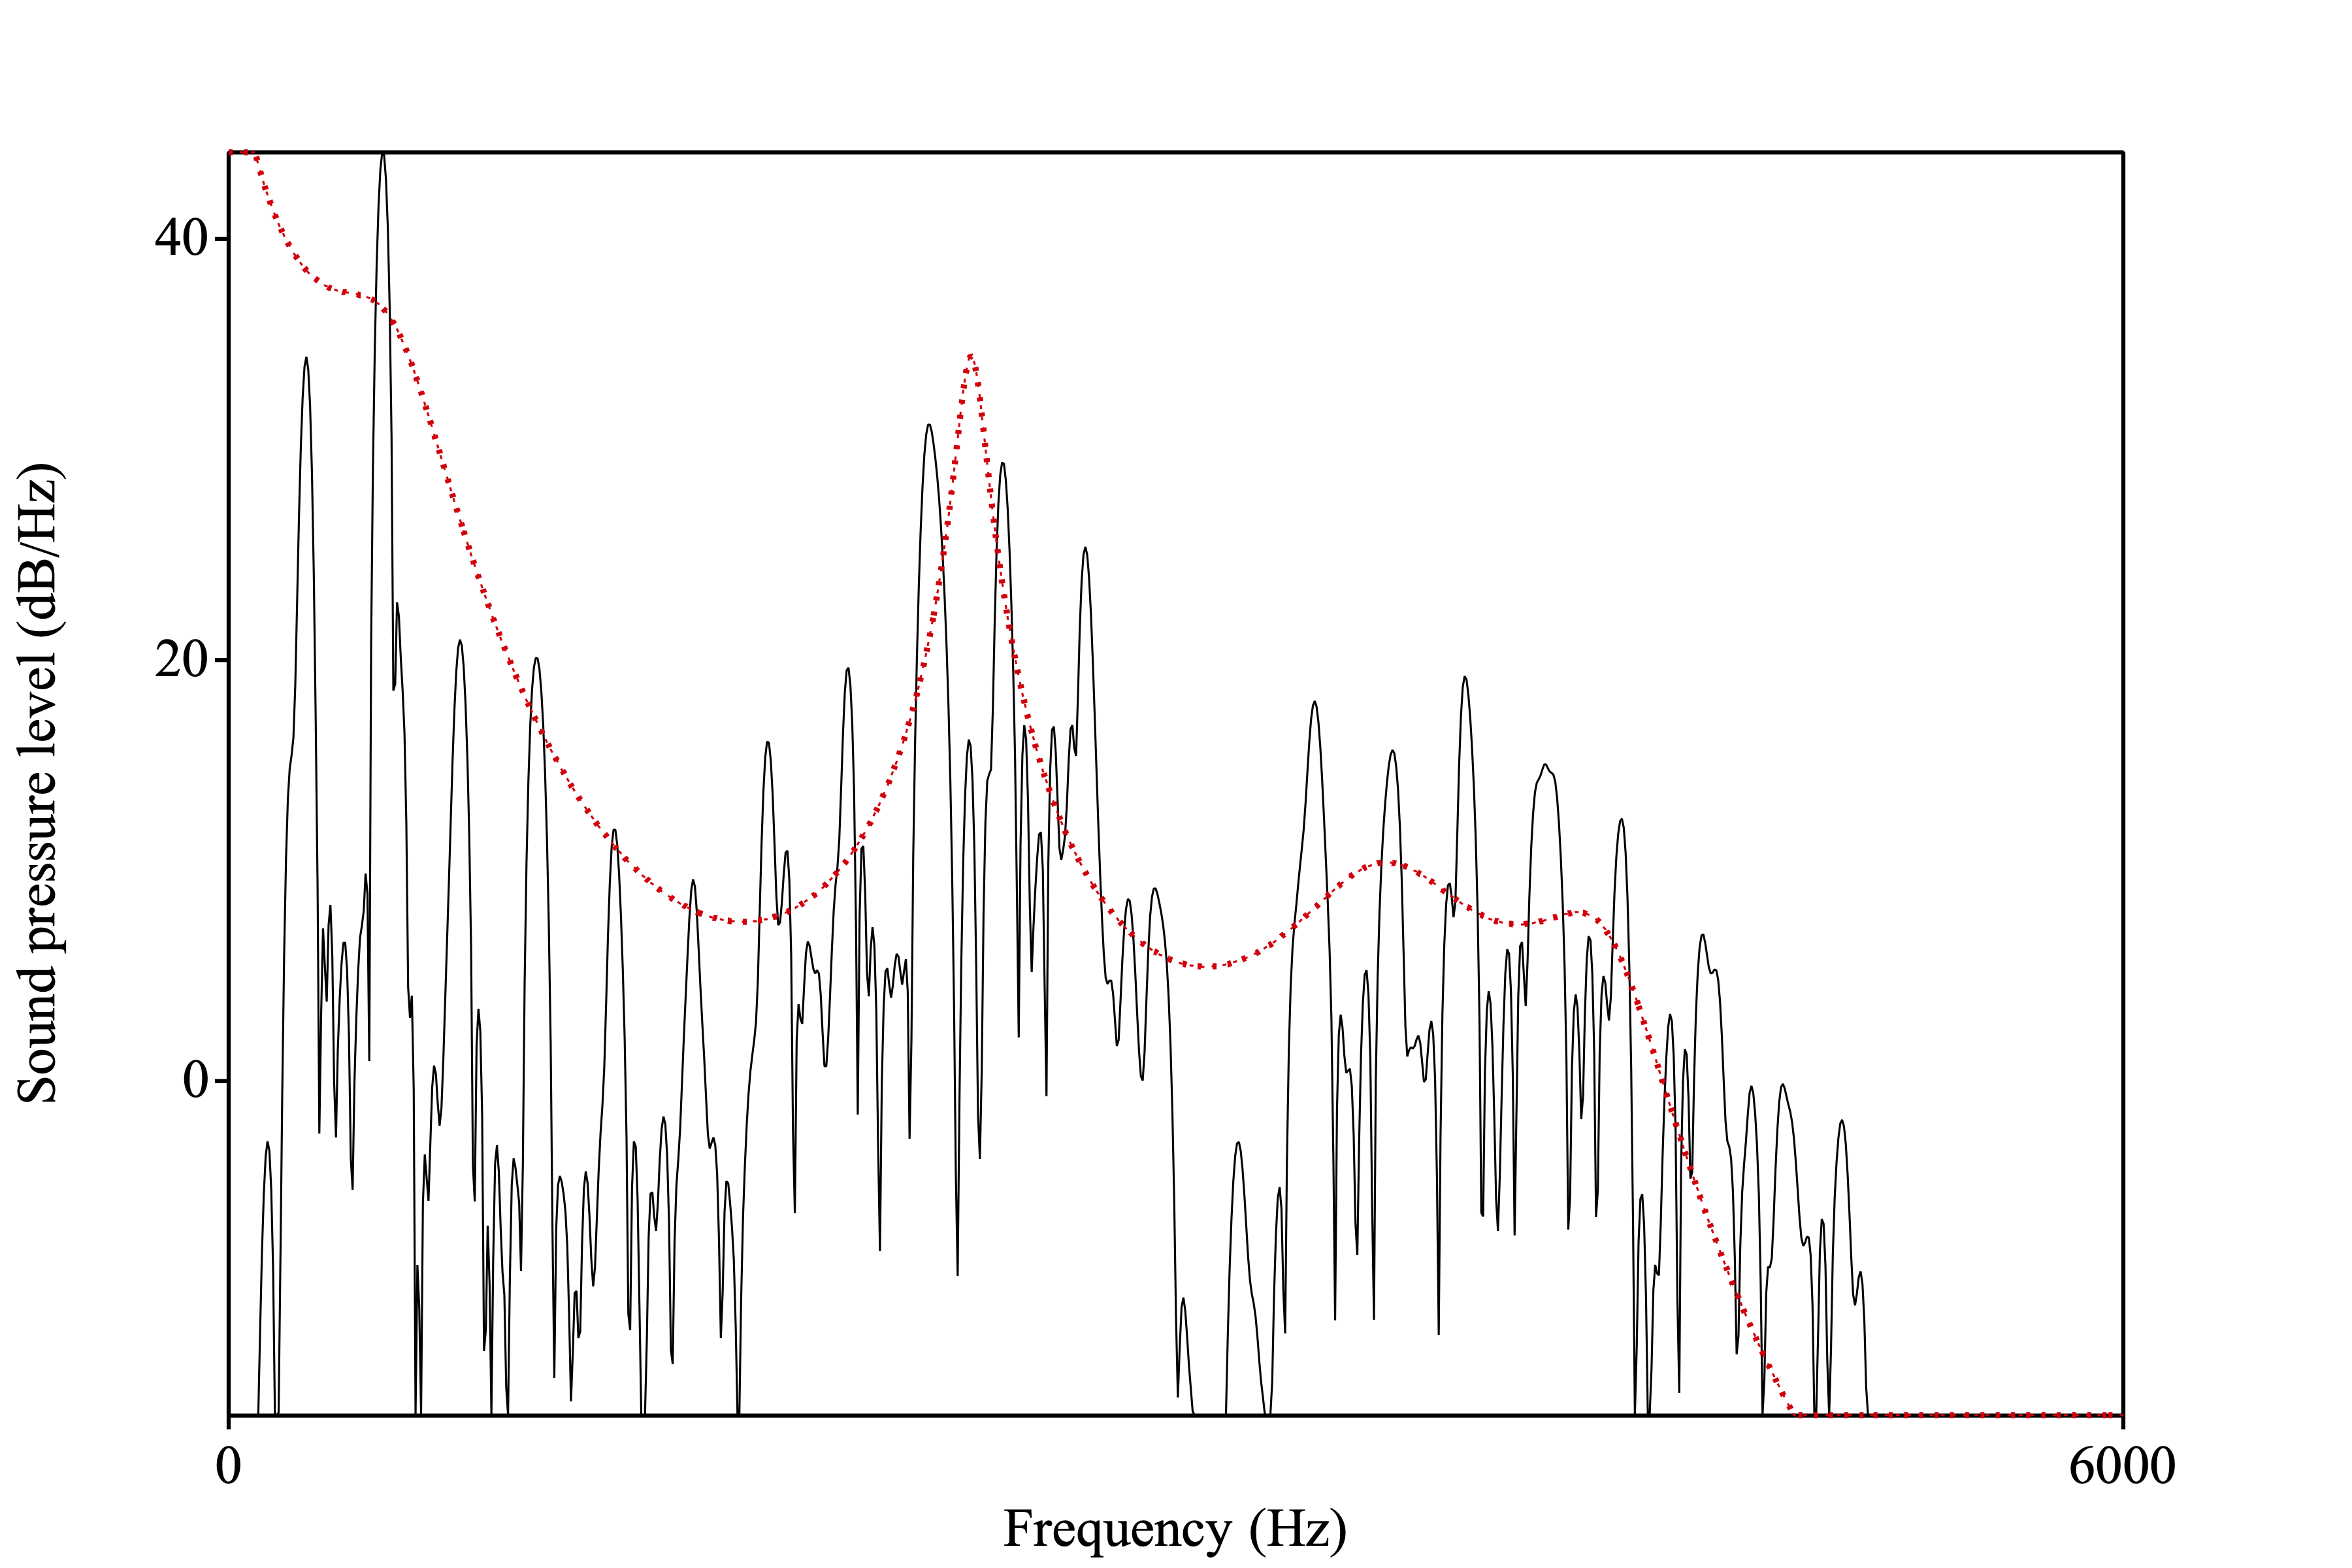
\includegraphics[width=0.9\textwidth]{Images/Harmonics.png}
	\caption{Spectral slice with LPC smoothed line overlaid for the vowel [e]. Each of the solid peaks represents the harmonics in the spectral slice. The leftmost black solid line peak is the first harmonic (H1), and each subsequent peak represents the next highest harmonic (H2 through H\textit{n}). The red dotted line represents an LPC smoothed line which identifies the formants by the peaks in the line.}
	\label{fig:Harmonics}
\end{figure}

From these studies, several patterns have emerged (see \cite{garellekPhoneticsVoice2019} for an overview). When interpreting the results of these spectral-tilt measures, several general patterns correspond to the different phonation types. For example, vowels produced with a breathy phonation typically have a higher spectral-tilt measurement when compared to vowels produced with modal phonation, and vowels produced with creaky phonation typically have a lower spectral-tilt measurement than modal vowels. 

In addition to spectral-tilt measurements, noise measurements frequently accompany phonation investigations (e.g., \cite{garellekPhoneticsWhiteHmong2021}). 

One of the most commonly used of these noise measurements is Cepstral Peak Prominence (CPP; \cite{hillenbrandAcousticCorrelatesBreathy1994,hillenbrandAcousticCorrelatesBreathy1996}). CPP is similar to the harmonics-to-noise ratio measure of \citet{dekromCepstrumBasedTechniqueDetermining1993} but differs in how the ‘prominence’ of the cepstral peak is calculated. Prominence is taken as the difference in amplitude of the cepstral peak, and a regression line is used to normalize window size and overall energy. In interpreting the measurement, a more prominent cepstral peak indicates stronger harmonics above the spectrum floor (i.e., greater periodicity in the speech signal). CPP was originally used as a diagnostic for breathy or modal voice \citep{blankenshipTimingNonmodalPhonation2002,espositoVariationContrastivePhonation2010} In fact, \citeauthor{espositoEffectsLinguisticExperience2010} showed that CPP was the best of the eight measures she considered for distinguishing modal from breathy phonation types. Further research has shown that CPP is also a good measurement for any non-modal phonation (e.g., \cite{andruskiPhonationTypesProduction2000,andruskiToneClarityMixed2006,blankenshipTimingNonmodalPhonation2002,waylandAcousticCorrelatesBreathy2003,avelinoAcousticElectroglottographicAnalyses2010}). 

%------------------------------------
\subsection{Psychoacoustic Model for Phonation} \label{sec:PMoP}
%------------------------------------

The \textsc{Psychoacoustic Model for Phonation} (PMoP; \cite{kreimanUnifiedTheoryVoice2014}) is a theoretical and clinical framework that addresses the problems that linguistics and speech pathologists face when working with phonation. The PMoP was designed to assist linguists and clinicians in understanding phonation from the perspectives of production and perception. The goals of this framework are: (i) link perception to acoustics by explaining quality in terms of perceptually valid acoustic measures that combine to determine voice quality fully; (ii) link voice production to acoustics and perception by determining which changes in the physiological voice source produced perceptible changes in the acoustic signal; and (iii) iterate until the two sets of acoustic parameters align. \citeauthor{kreimanUnifiedTheoryVoice2014} 

\begin{table}[!h]
    \centering
    \caption{Components of the psychoacoustic model of voice quality and associated parameters (from \cite{kreimanUnifiedTheoryVoice2014}).}
    \label{tab:Kreiman}
    \begin{tabular}{ll}
    \lsptoprule
    Model component & Parameters \\
    \hline
    Harmonic source spectral slope      & H1-H2 \\
                                        & H2-H4 \\
	                                & H4-H2k Hz \\
	                                & H2k Hz-H5k Hz \\
    Inharmonic source noise             & Harmonics-to-noise ratio \\
    Time-varying source characteristics & $f_0$ track \\
	                                & Amplitude track \\
    Vocal tract transfer function       & Formant frequencies and bandwidths \\
	                                & Spectral zeros and bandwidths\\
    \lspbottomrule
    \end{tabular}
\end{table}


%------------------------------------
\section{Phonation contrasts in Santiago Laxopa Zapotec} \label{sec:SLZ}
%------------------------------------

Santiago Laxopa Zapotec (SLZ; \textit{Dilla'xhunh Laxup}) is a Northern Zapotec language spoken by approximately 1000 people in the municipality of Santiago Laxopa, Ixtlán District in the Sierra Norte of Oaxaca, Mexico \citep{adlerAcousticsPhonationTypes2016,adlerDerivationVerbInitiality2018,foleyForbiddenCliticClusters2018,foleyExtendingPersonCaseConstraint2020}. It is mutually intelligible with San Bartolomé Zoogocho Zapotec \citep{longDiccionarioZapotecoSan2005,sonnenscheinDescriptiveGrammarSan2005}. SLZ has a fairly standard five-vowel inventory; see Table~\ref{tab:SLZvowels}.

\begin{table}[!h]
\centering
\caption{Vowels inventory in Santiago Laxopa Zapotec.}
\label{tab:SLZvowels}
    \begin{tabular}{lccc}
    \lsptoprule
	&  front& central  & back \\
    \midrule
    high   	&  i  &     &   u \\
    mid    	&  e  &   	& 	o \\
    low   	&     &  a 	&	  \\
    \lspbottomrule
    \end{tabular}
\end{table}
		
Among Zapotecan languages, it is quite common for languages to make use of contrastive phonation \citep[e.g.,][]{avelinobecerraTopicsYalalagZapotec2004,longDiccionarioZapotecoSan2005,avelinoAcousticElectroglottographicAnalyses2010,lopeznicolasEstudiosFonologiaGramatica2016,chavez-peonInteractionMetricalStructure2010}. 
SLZ, in addition to the five vowel qualities mentioned above, has four contrastive phonation types: modal, breathy, checked, and laryngealized. These contrasts are exemplified in the minimal quadruple in (\ref{ex:YA}).

In representing the checked and laryngealized vowels, I follow the same procedure as other authors (e.g., \citet{avelinoAcousticElectroglottographicAnalyses2010, uchiharaToneRegistrogenesisQuiavini2016}) in representing the `glottal stop' element as a superscript glottal stop in the IPA transcription (i.e., [aˀ]). This is primarily done as a way of standardizing the variable pronunciation of the glottal element in Zapotec, ranging from a full glottal stop (i.e., [aʔ]) to a creaky portion of the vowel (i.e., [aa̰]).  

\ea \label{ex:YA} Four-way near minimal phonation contrast
    \ea \textit{yag}  /çag\supr{L}/ `tree; wood; almúd (unit of measurement approximately 4kg)'
    \ex \textit{yah}  /ça̤\supr{L}/ `metal; rifle; bell'
    \ex \textit{yu'}  /çuˀ\supr{L}/  `earth'
    \ex \textit{ya'a}  /çaˀa\supr{L}/  `market'
    \z 
\z 

Breathy phonation on vowels is characterized by a raspy quality throughout the whole vowel or a portion toward the end of the vowel; see Figure~\ref{fig:BreathyVowel}. 

\begin{figure}[!h]
	\centering
	% [INSERT YAH SPECTROGRAM AND WAVEFORM]
	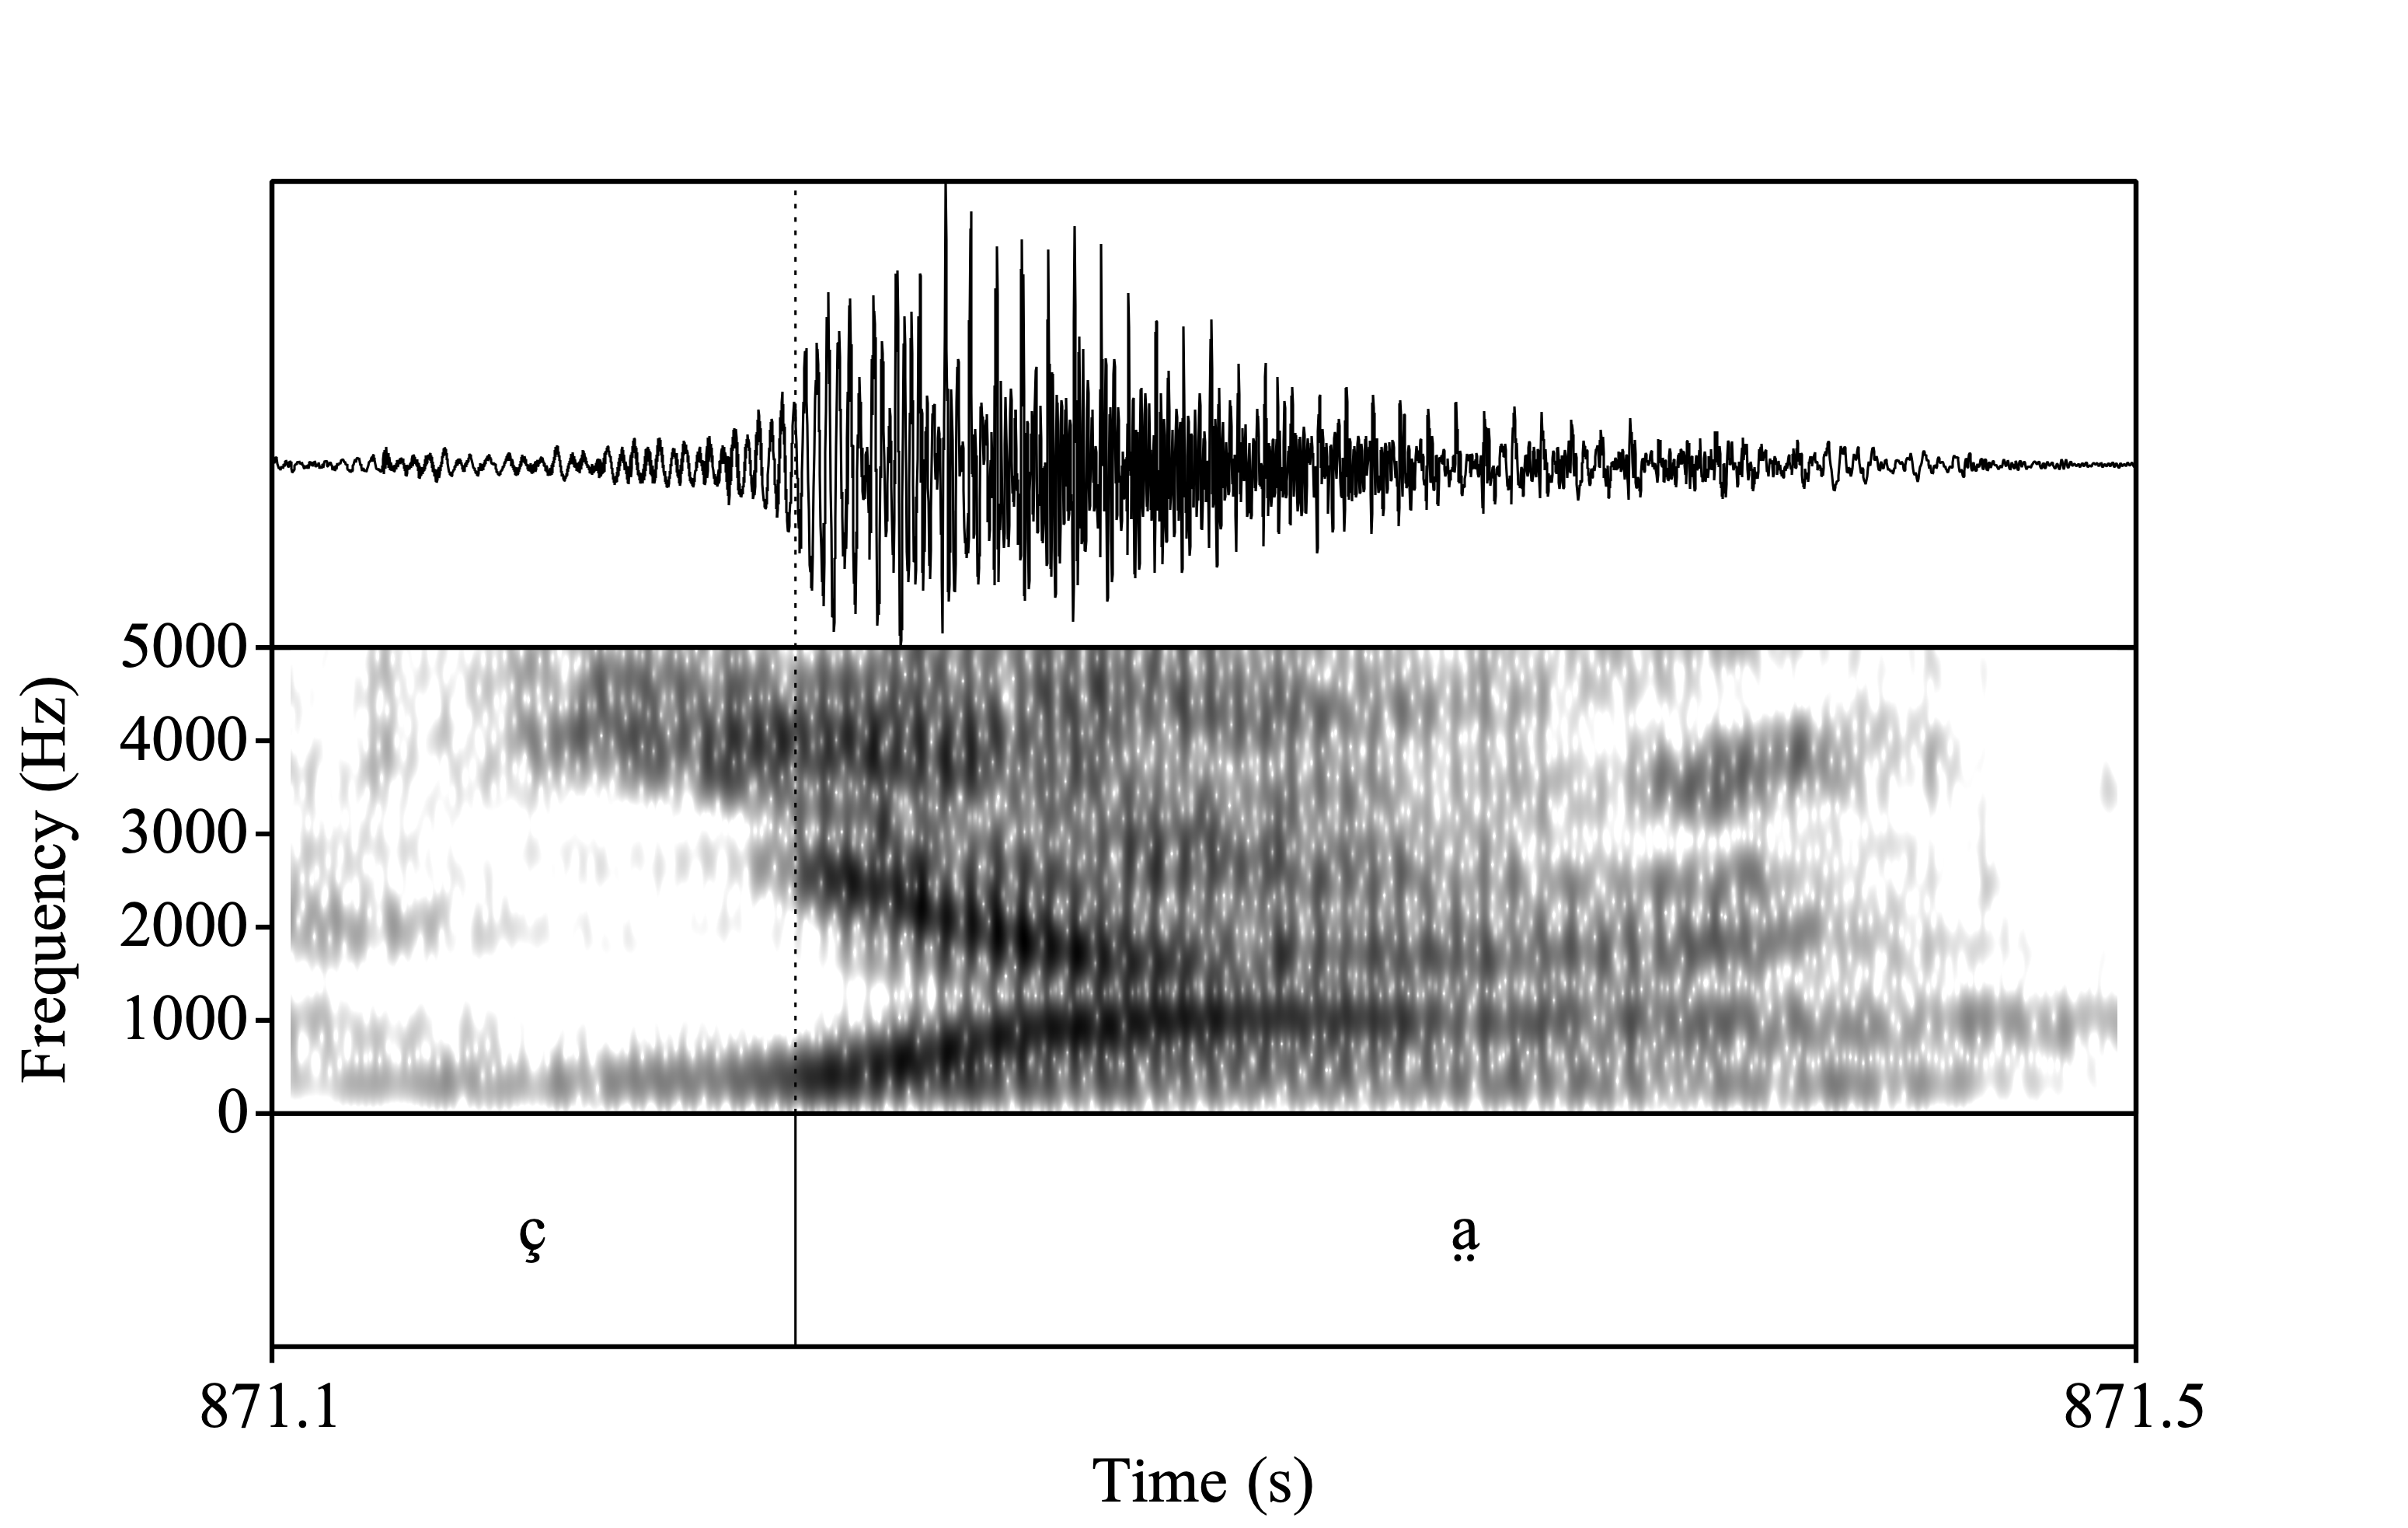
\includegraphics[width=0.9\textwidth]{Images/yah.png}
	\caption{Breathy vowel in the word \textit{yah} `metal; rifle'}
	\label{fig:BreathyVowel}
\end{figure}

On the other hand, checked vowels are characterized by an abrupt glottal closure which cuts the vowel short. This phonation is sometimes only realized as a very short period of creakiness at the end of the vowel; see Figure~\ref{fig:CheckedVowel}.  

\begin{figure}[!h]
	\centering
	% [INSERT YA SPECTROGRAM AND WAVEFORM]
	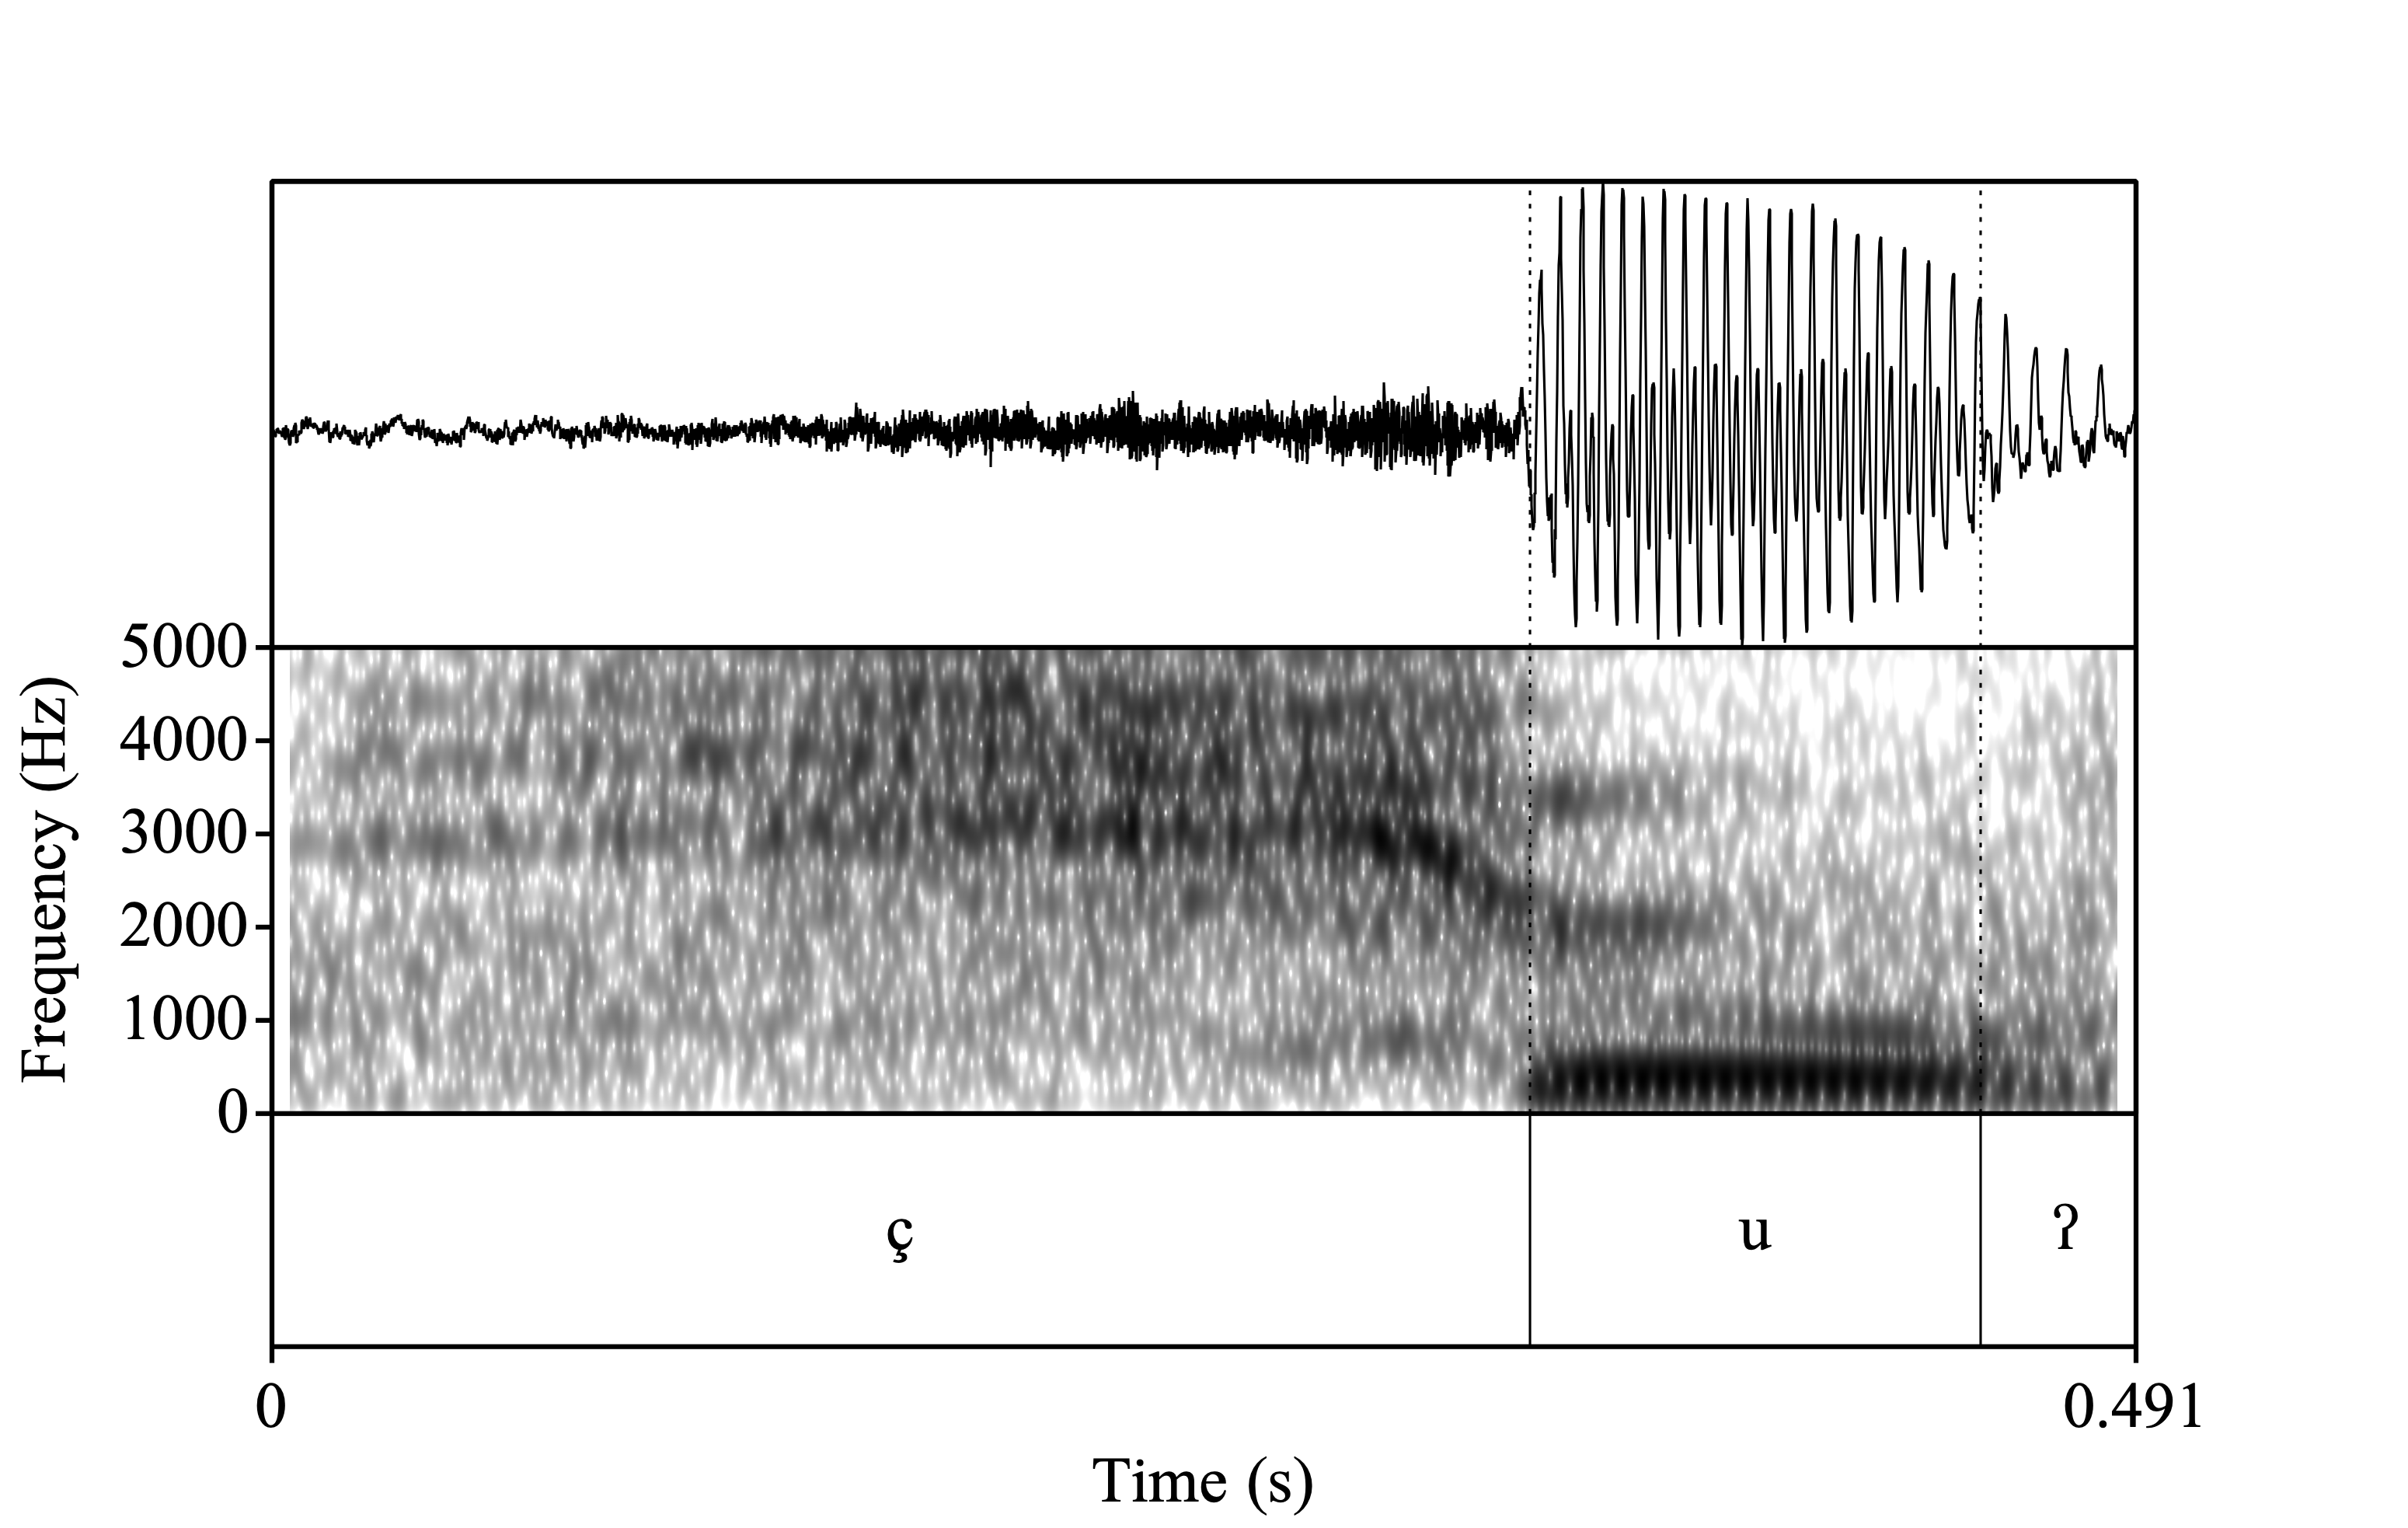
\includegraphics[width=0.9\textwidth]{Images/RD_yu'.png}
	\caption{Checked vowel in the word \textit{yu'} `earth'}
	\label{fig:CheckedVowel}
\end{figure}

Laryngealized vowels are common in Zapotecan languages and have received many names. Previous descriptions have used terms such as broken, rearticulated, interrupted, and creaky to describe this phonation type \citep{longDiccionarioZapotecoSan2005,avelinobecerraTopicsYalalagZapotec2004,avelinoAcousticElectroglottographicAnalyses2010,sonnenscheinDescriptiveGrammarSan2005,adlerAcousticsPhonationTypes2016}. To avoid confusion; I will use the term laryngealized following \citet{avelinoAcousticElectroglottographicAnalyses2010}. In addition to many different names, these vowels exhibit a wide range of allophones. 

\citet{avelinoAcousticElectroglottographicAnalyses2010} found in the closely related Yalálag Zapotec that among his consultants, there were at least four different pronunciations as seen in Table~\ref{tab:laryngeal}. 
\begin{table}[!h]
	\centering
	\caption{Layngealized Vowels in Yalálag Zapotec}
	\label{tab:laryngeal}
	 \begin{tabular}{ll}
	\lsptoprule
	/VˀV/	&  [VʔV]  \\
			&  [VV̰V]   \\
			&  [VV̰ːV̆]  \\
			&  [VV̰V̰]	\\
	\lspbottomrule
	\end{tabular}
\end{table}
In SLZ, each consulted language expert would produce this vowel differently. One consultant would re-articulate with a full glottal stop in the middle of the vowel, or they would produce creaky voice. This alternation seemed to be in free variation, but there was a greater tendency to creak in low-toned words, such as \textit{xa'ag} [ʂa̰ːg] `topil'\footnote{A \textit{topil} is a type of government office in traditional Oaxacan communities somewhat akin to a sheriff.}, see Figure~\ref{fig:FSRLaryngeal} for a comparison between this consultant's pronunciation of the laryngealized vowels.

\begin{figure}[!h]
	\centering
	\begin{subfigure}{.5\textwidth}
		\centering
		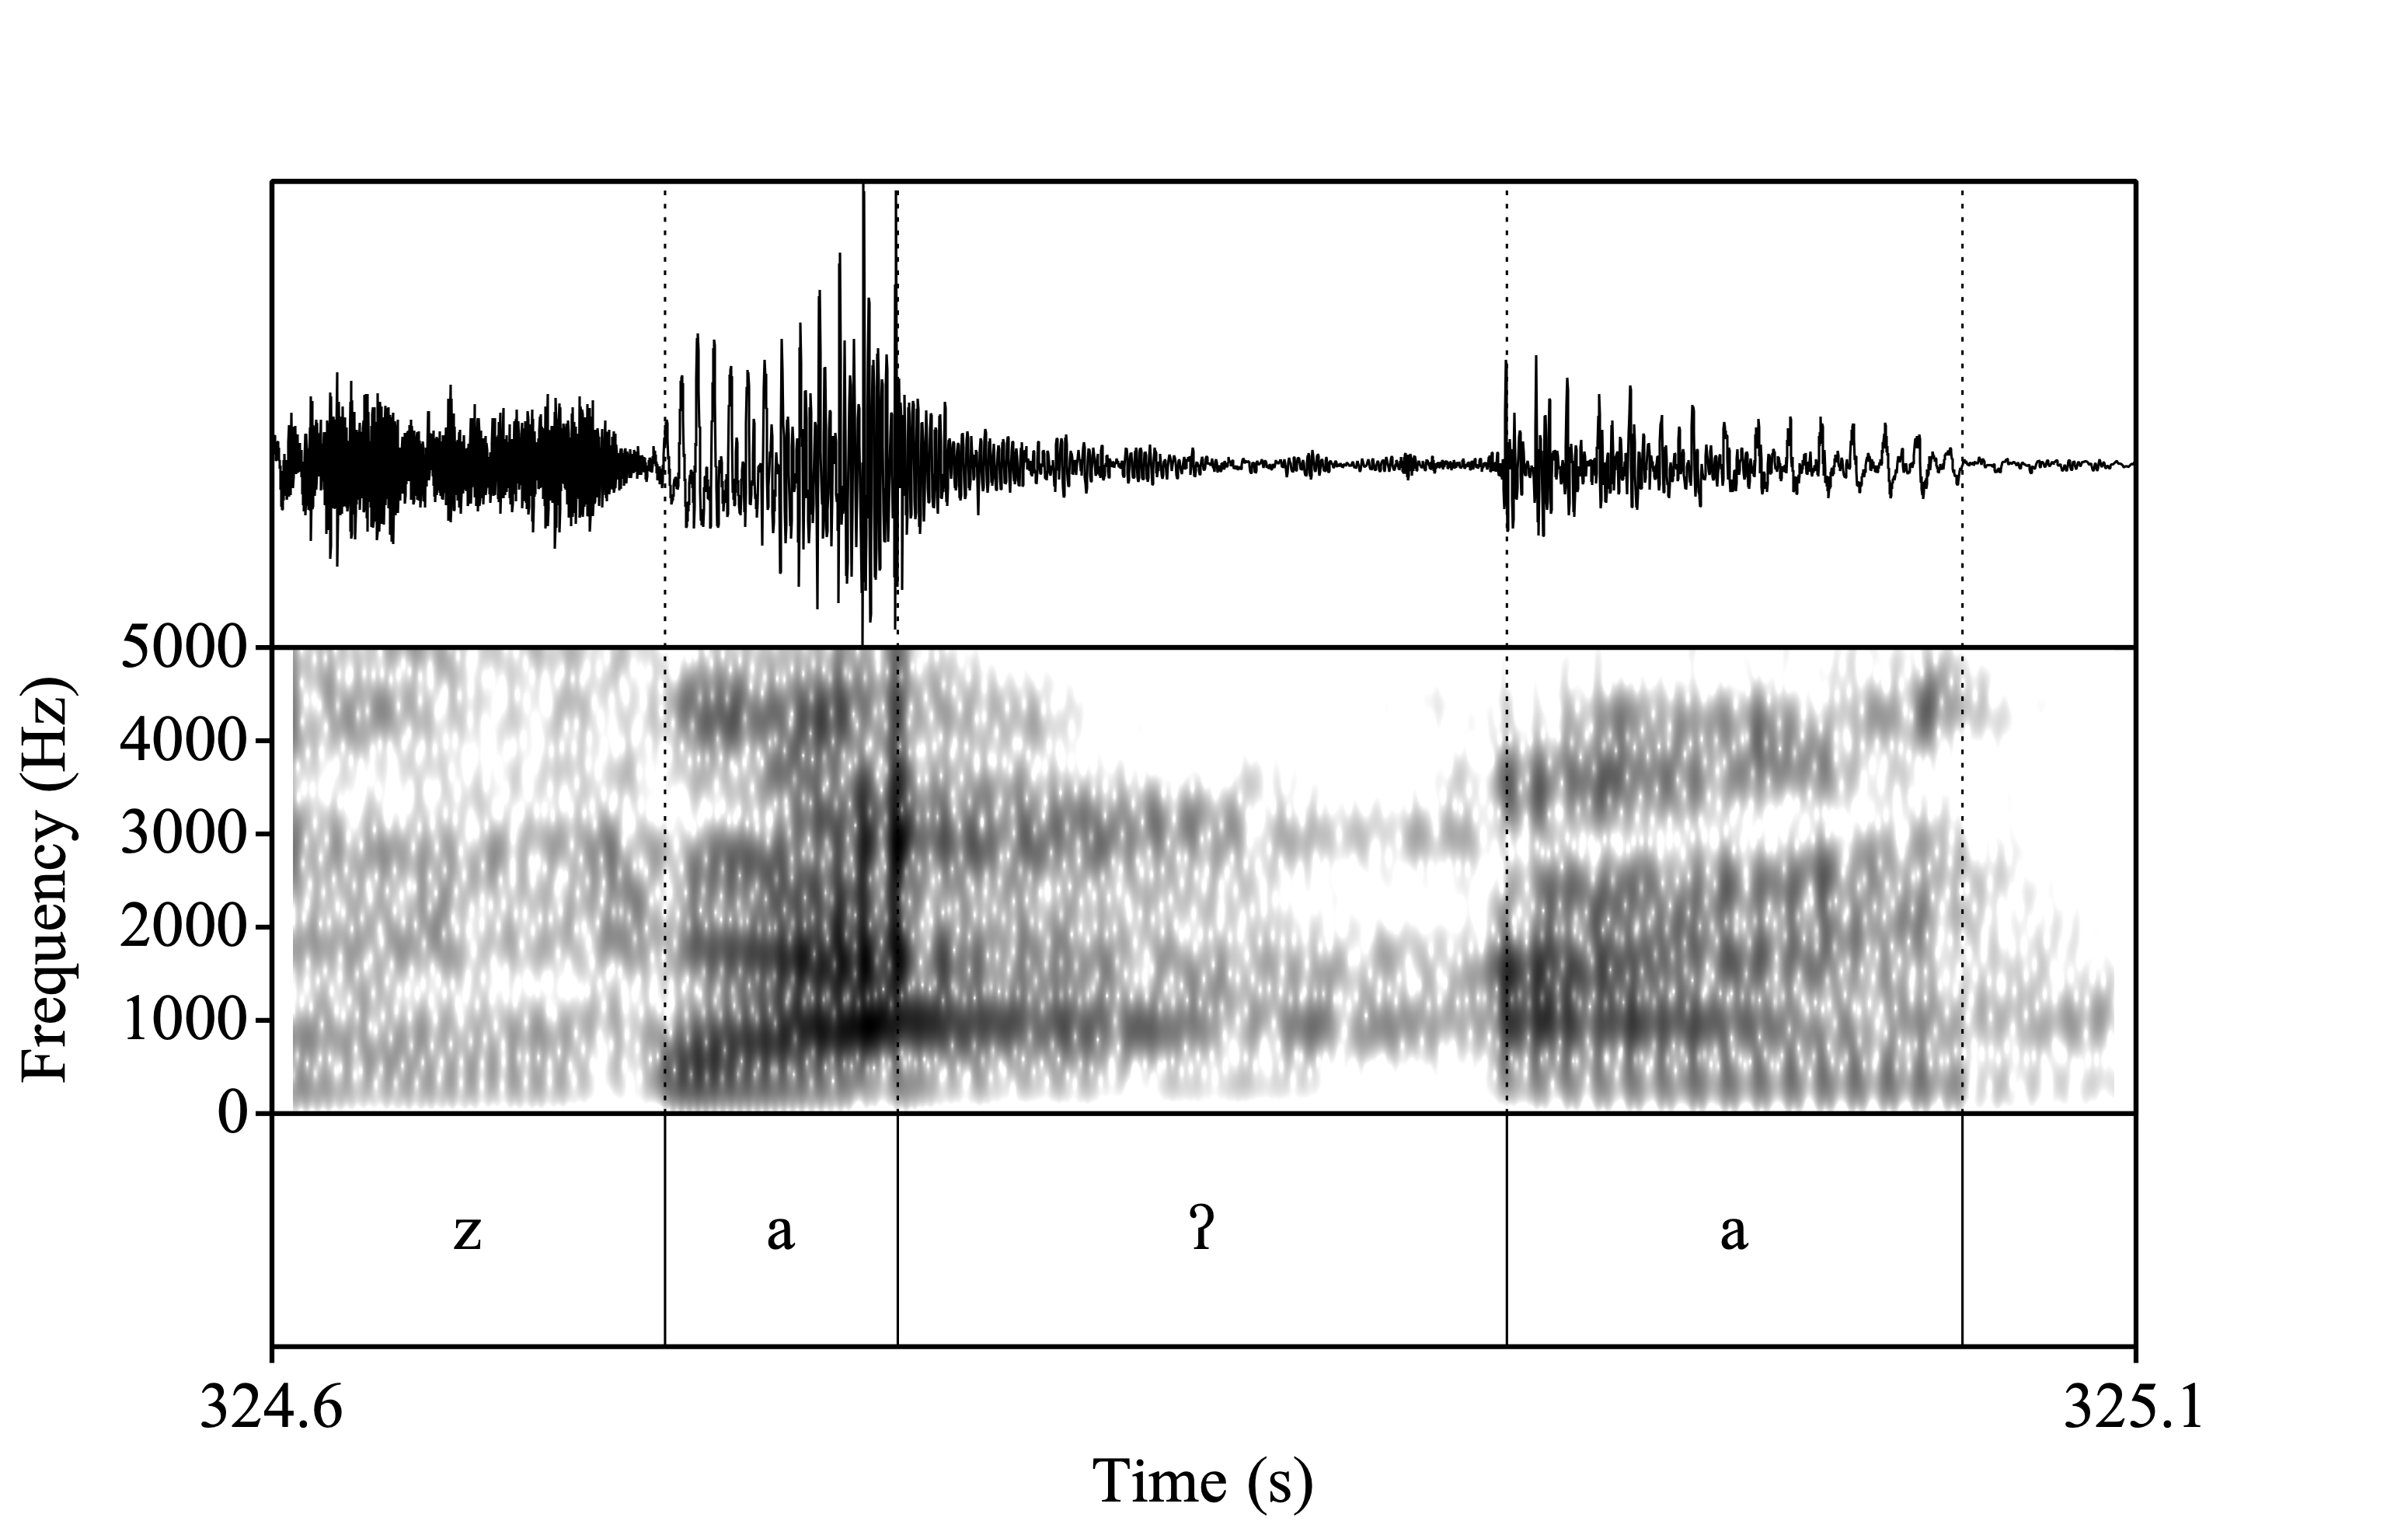
\includegraphics[width=\linewidth]{Images/za'a.png}
		\caption{\textit{za'a} `corncob'}
		\label{fig:FSRza'a}
	\end{subfigure}%
	\begin{subfigure}{.5\textwidth}
		\centering
		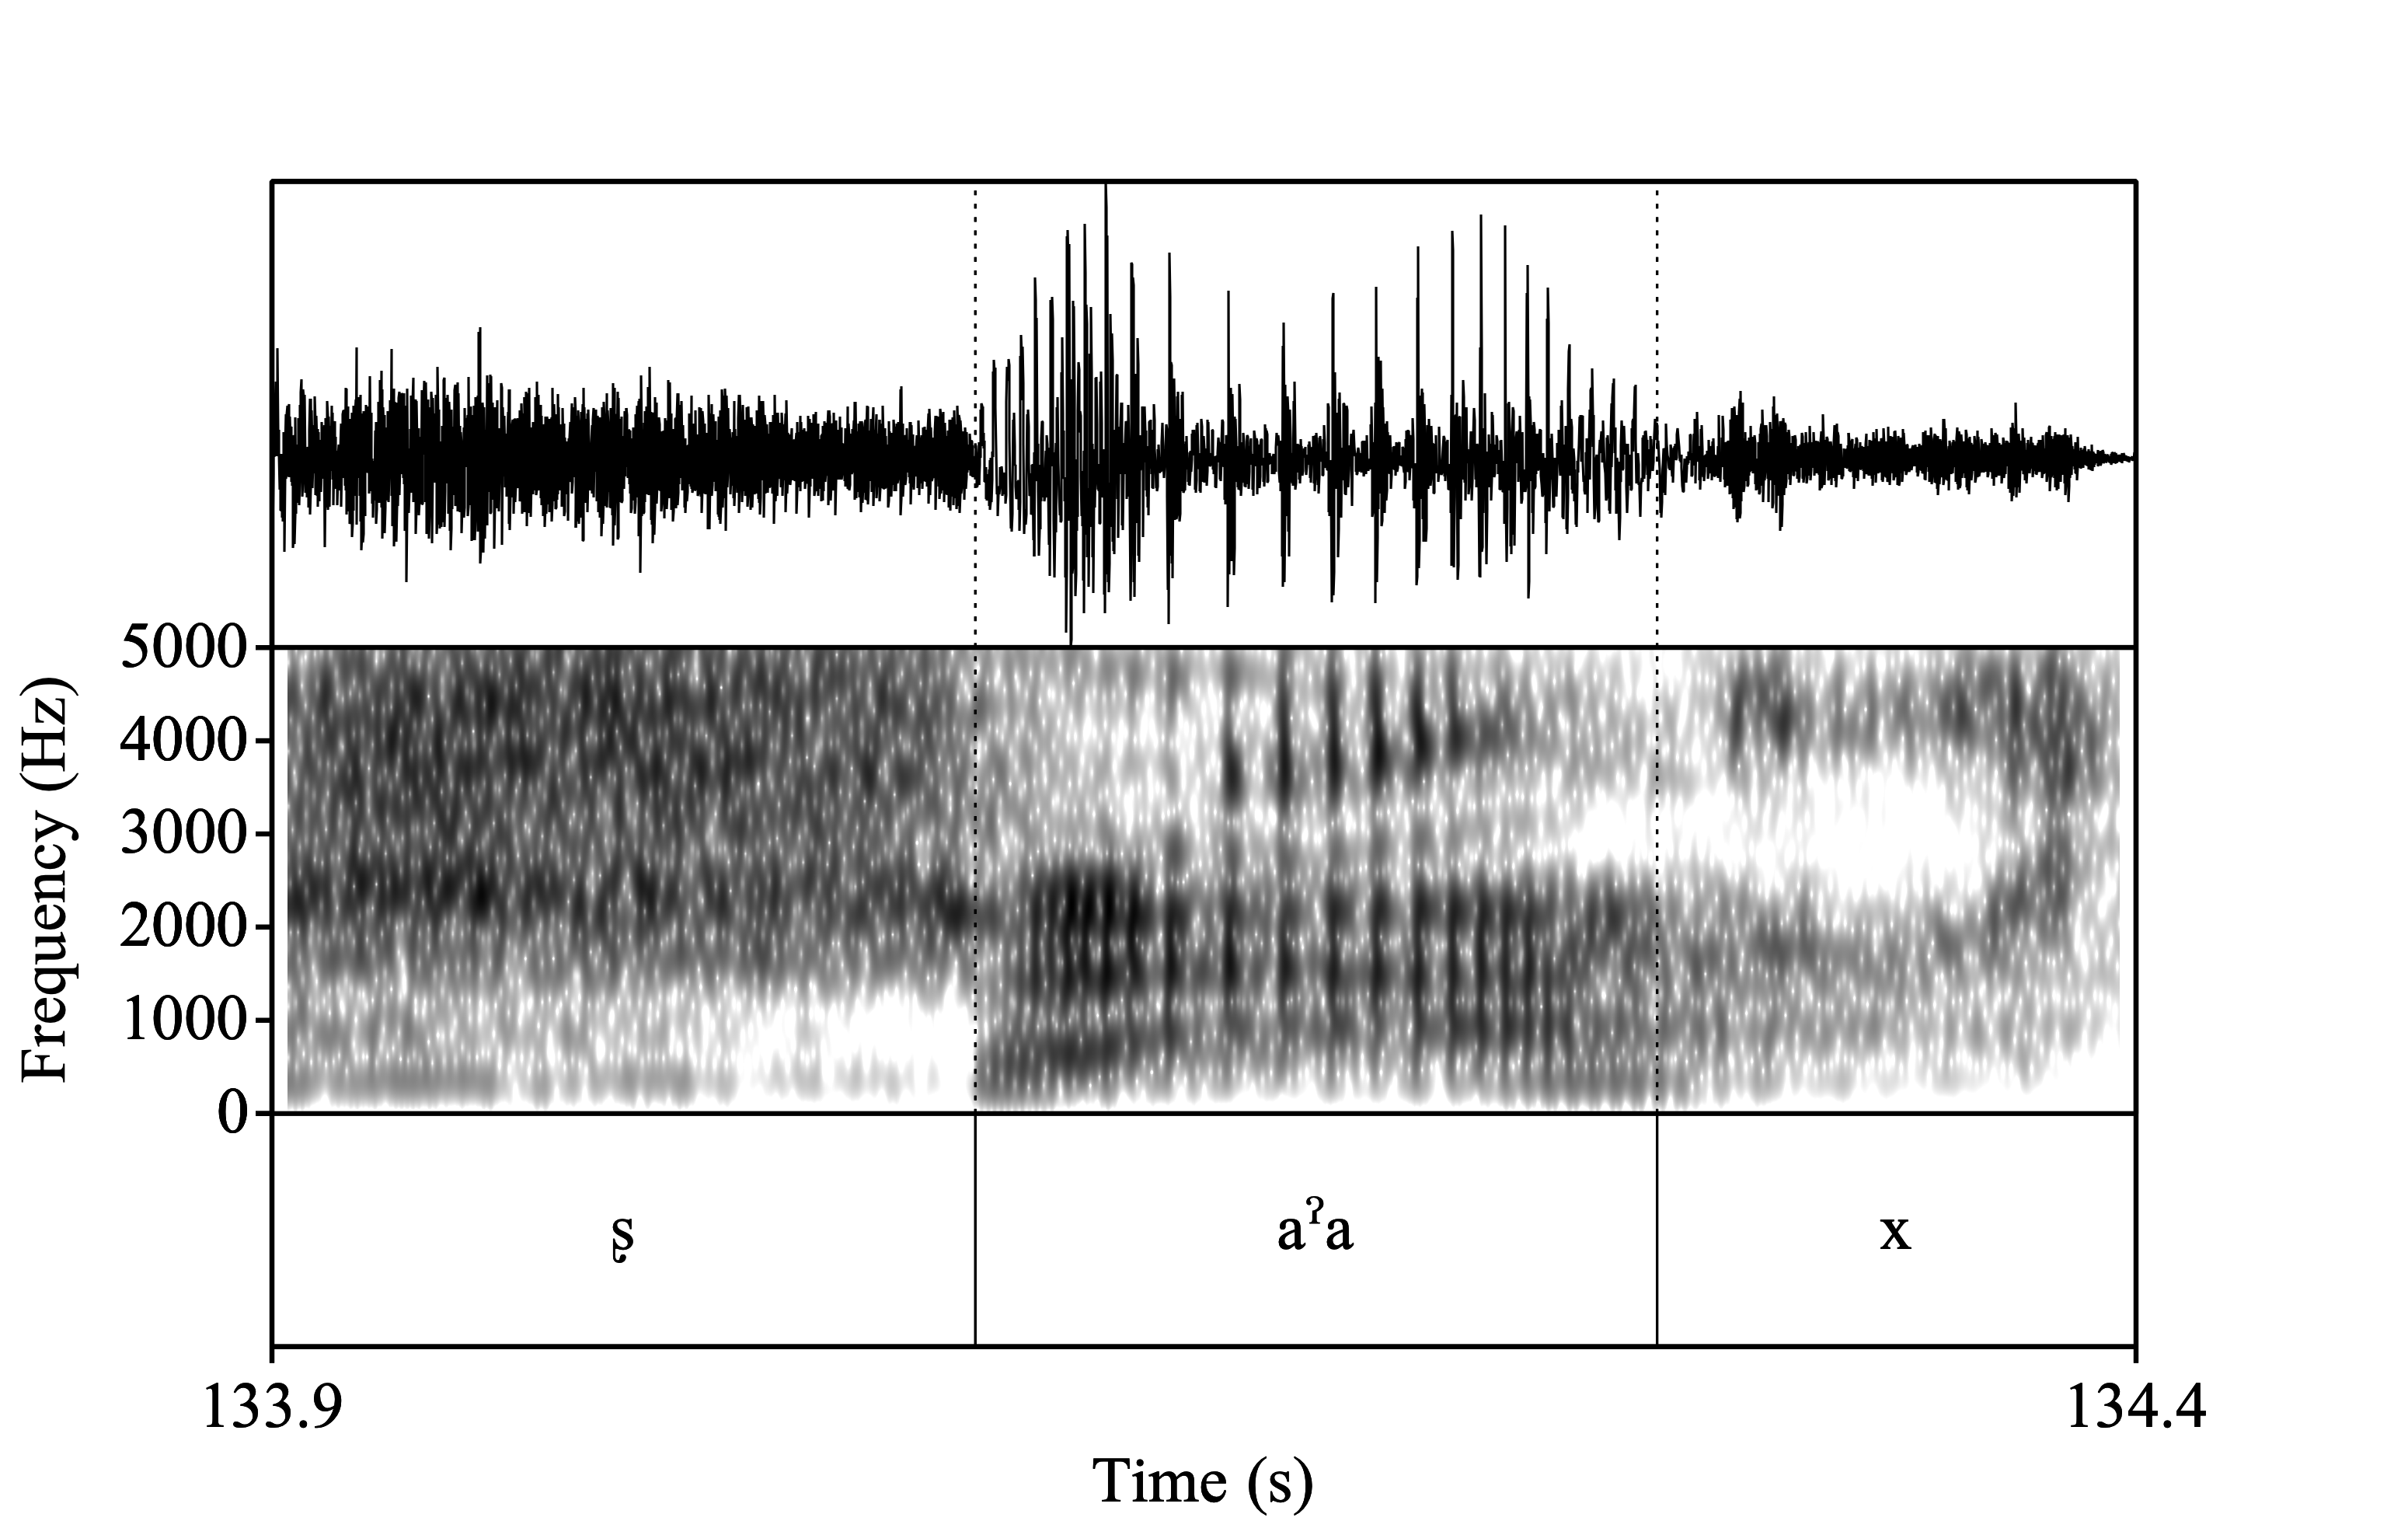
\includegraphics[width=\linewidth]{Images/xa'ag.png}
		\caption{\textit{xa'ag} `topil'}
		\label{fig:FSRxa'ag}
	\end{subfigure}	
	\caption{Comparison of FSR's laryngealized vowels in \textit{za'a} `corncob' and \textit{xa'ag} `topil'}
	\label{fig:FSRLaryngeal}
\end{figure}

The other consultant only produces creaky voice for these vowels regardless of the tone of the word. During one of the elicitation sessions, we conducted a perceptual check that these were, in fact, the same vowels, and both consultants reliably identified the words. They produced laryngealized vowels according to their own idiosyncrasies. However, a more detailed perception study is beyond the scope of this paper. 
\begin{figure}[!h]
	\centering
	\begin{subfigure}{.5\textwidth}
		\centering
		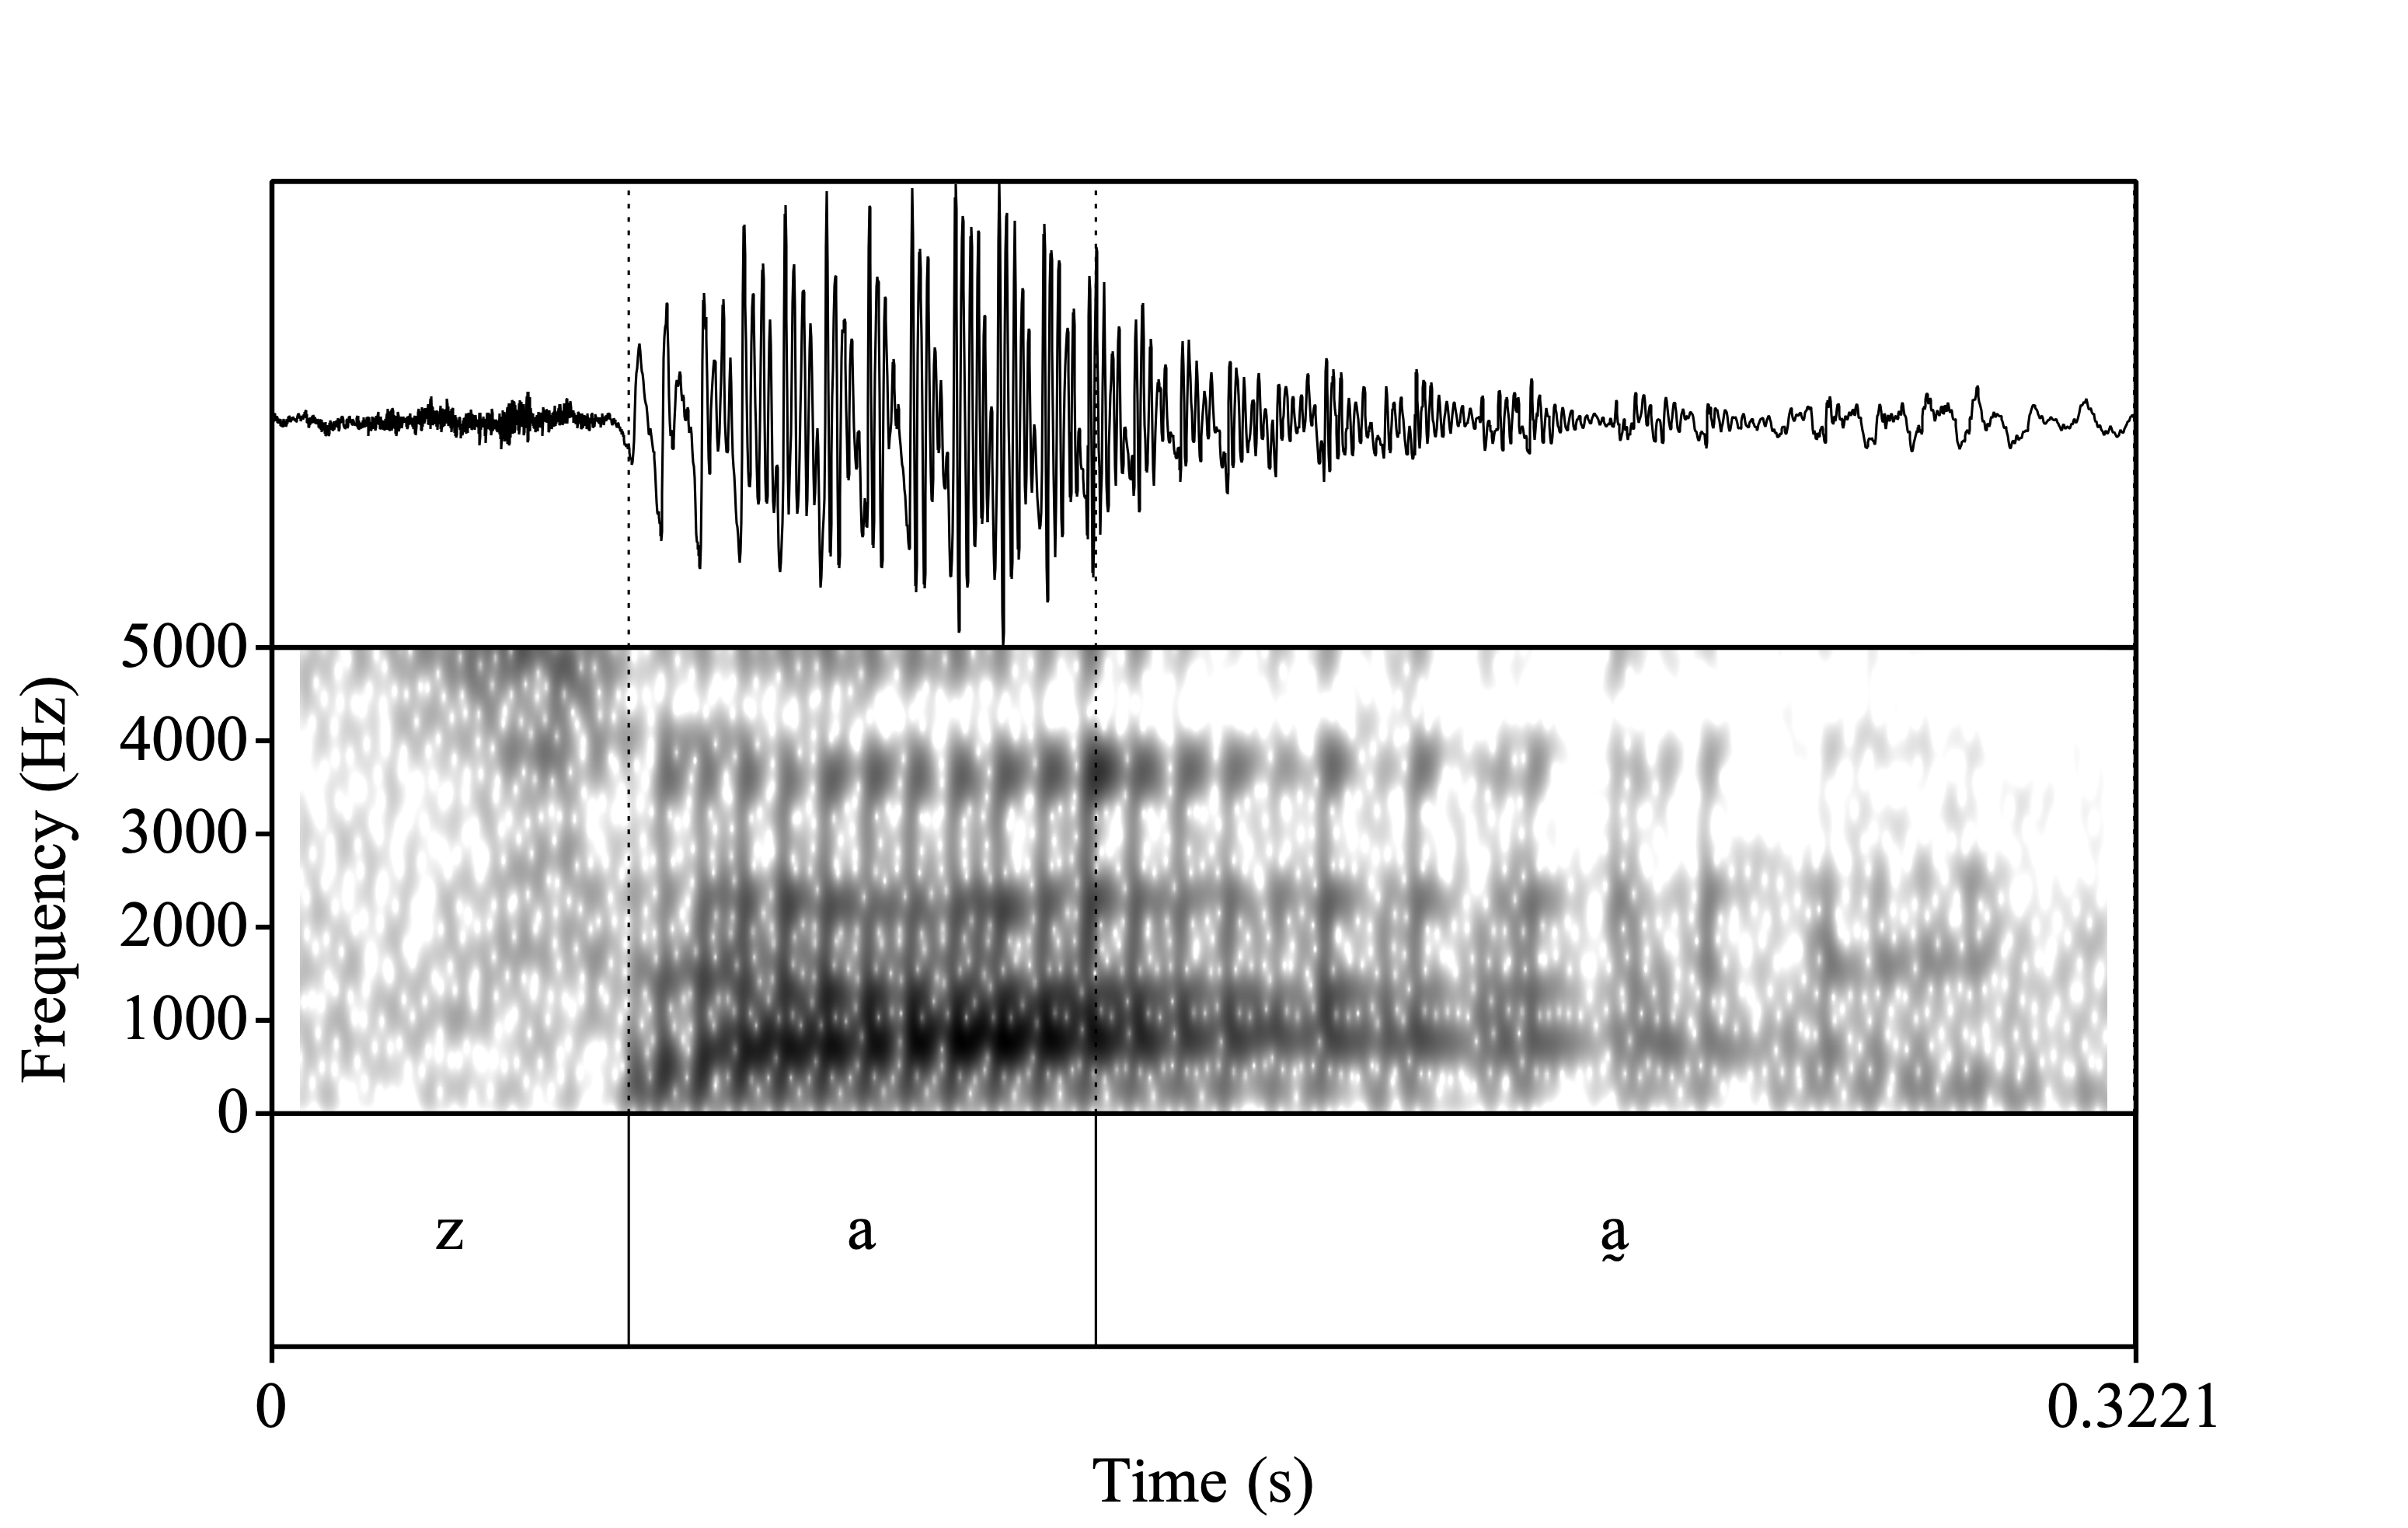
\includegraphics[width=\linewidth]{Images/RD_za'a.png}
		\caption{\textit{za'a} `corncob'}
		\label{fig:RDza'a}
	\end{subfigure}%
	\begin{subfigure}{.5\textwidth}
		\centering
		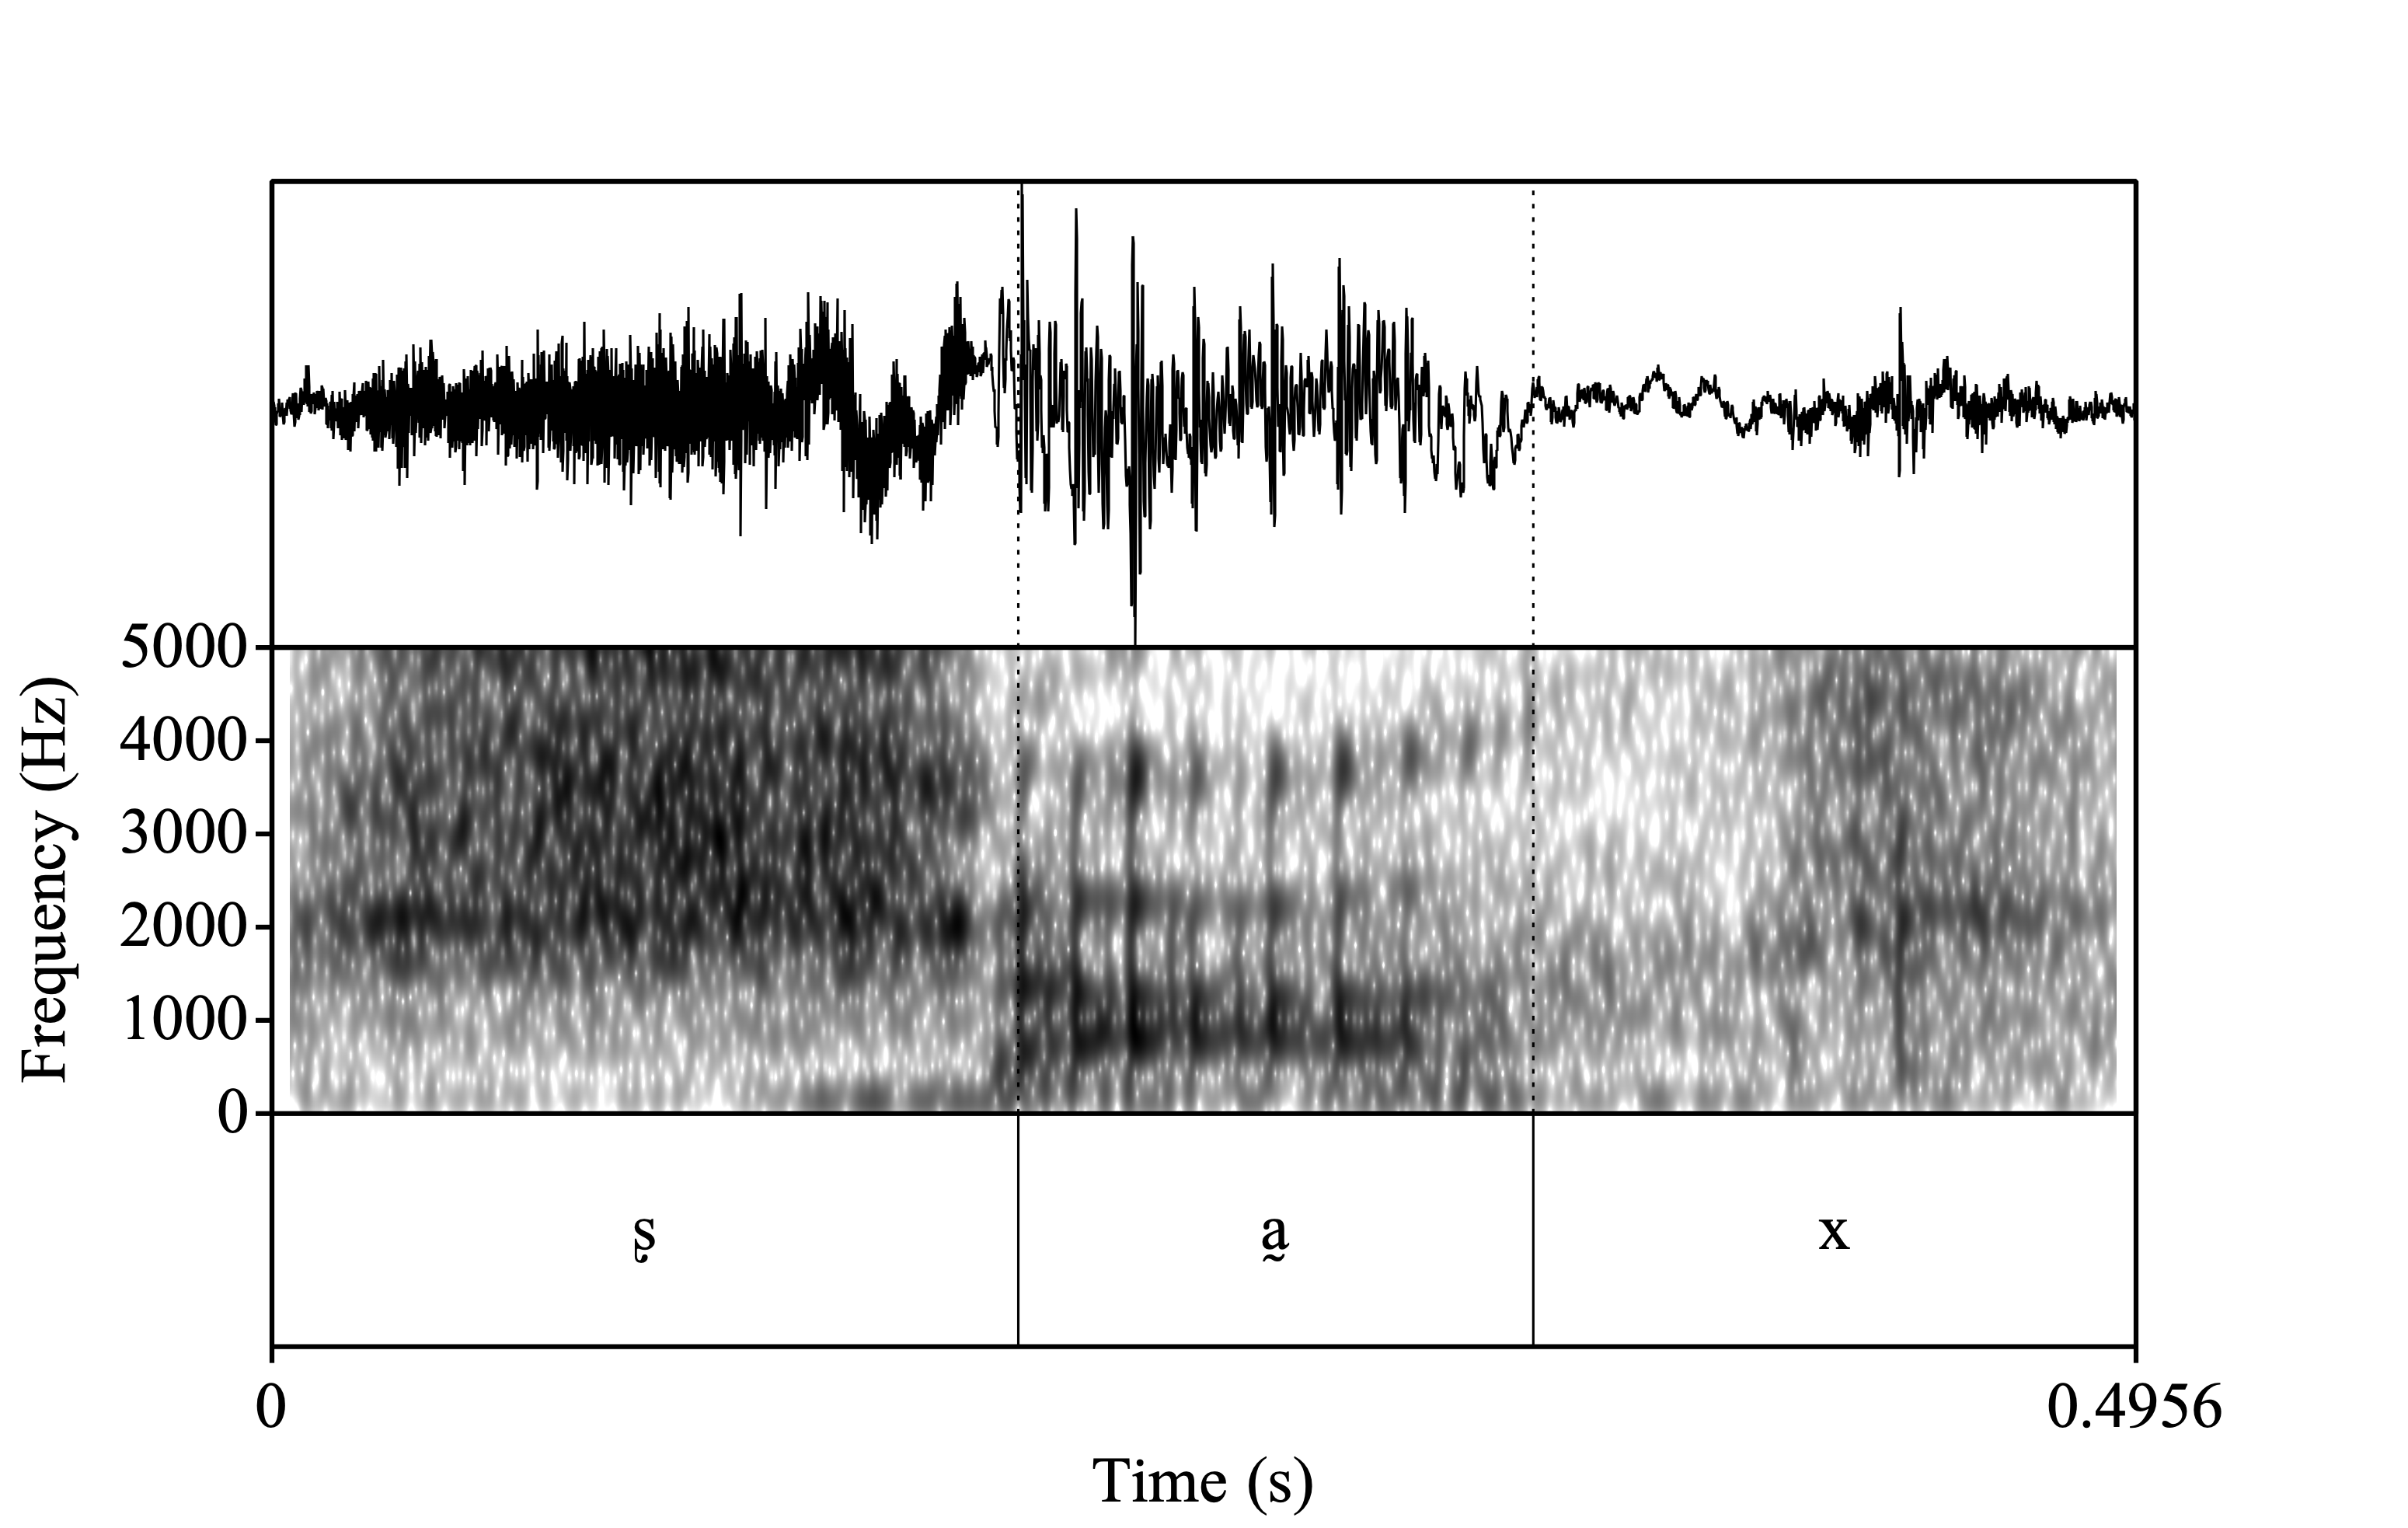
\includegraphics[width=\linewidth]{Images/RD_xa'ag.png}
		\caption{\textit{xa'ag} `topil'}
		\label{fig:RDxa'ag}
	\end{subfigure}
	\caption{Comparison of RD's laryngealized vowels in \textit{za'a} `corncob' and \textit{xa'ag} `topil'}
	\label{fig:RDLaryngeal}
\end{figure}

%------------------------------------
\subsection{Interaction of Tone and Phonation} \label{sec:Interaction}
%------------------------------------

Most previous work on the interaction of tone has been focused on the languages of East and Southeast Asia \citep[e.g.,][]{masicaDefiningLinguisticArea1976,thurgoodVietnameseTonogenesisRevising2002,yipTone2002,enfieldArealLinguisticsMainland2005,michaudComplexTonesEast2012,brunelleTonePhonationSoutheast2016}. What has been found in these descriptions is that certain tones and phonations are codependent. For example, \citet{smalleyProblemsConsonantsTone1976} and \citet{ratliffMeaningfulToneStudy1992} both describe White Hmong's \textit{-g} tone as being a mid-low tone with breathy phonation and Mandarin's tone 3 is often associated with creaky phonation \citep{hockettPeipingPhonology1947}. \citet{brunelleTonePerceptionNorthern2009} found that creaky phonation plays an important role in producing certain tones. Additionally, work on S'gaw Karen has found that two tones are only differentiated by some form of non-modal phonation (Boehm p.c.). 

However, there have been some observations–especially in Mesoamerica–that tone and phonation are independent of each other \citep[e.g.,][]{silvermanLaryngealComplexityOtomanguean1997,garellekAcousticConsequencesPhonation2011}. This means that tone can independently occur with any phonation type. This has also been extensively described in multiple Zapotecan languages \citep[e.g.,][]{,avelinobecerraTopicsYalalagZapotec2004,avelinoAcousticElectroglottographicAnalyses2010, chavez-peonInteractionMetricalStructure2010, campbellZenzontepecChatinoAspect2011,villardPhonologyMorphologyZacatepec2015, lopeznicolasEstudiosFonologiaGramatica2016}

\citet{chavez-peonInteractionMetricalStructure2010} describes the tone and phonation interactions in San Lucas Quiaviní Zapotec (SLQZ), a central valley variety of Zapotec. The distribution of tone and phonation is found in Table~\ref{tab:SLQZ}. We see that in SLQZ, both low- and falling-tones have the full range of possible combinations. However, we see gaps in the high-tone for breathy and rising tones that can only occur with modal phonation. 

\begin{table}[!ht]
	\centering
	\caption{SLQZ tone and phonation interactions \citep{chavez-peonInteractionMetricalStructure2010}.}
	\label{tab:SLQZ}
	 \begin{tabular}{lcccc}
	  \lsptoprule
					  &	 \textbf{Modal}  & \textbf{Breathy} & \textbf{Creaky} & \textbf{Interrupted} \\
		  High	& ✔︎ & -- & ✔︎ & ✔︎ \\
		  Low & ✔︎ & ✔︎ & ✔︎ & ✔︎ \\
		  Falling & ✔︎ & ✔︎ & ✔︎ & ✔︎ \\
		  Rising & ✔︎ & -- & -- & -- \\
	  \lspbottomrule
	 \end{tabular}
\end{table}

Based on elicitation data collected from 2020-2022, SLZ has a more expansive distribution of tone and phonation when compared to SLQZ but seems to be very similar to other Northern Zapotec varieties \citep[e.g.,][]{avelinobecerraTopicsYalalagZapotec2004}. The distribution of SLZ tonal and phonation interactions are given in Table~\ref{tab:ToneVoiceQuality} for the number of analyzed tokens. 
\begin{table}[!h]
	\caption{SLZ tone and phonation interactions.}
	\label{tab:ToneVoiceQuality}
	\centering

	\begin{tabular}{lcccc}
	\lsptoprule
		& \textbf{Modal} & \textbf{Breathy} & \textbf{Checked} & \textbf{Laryngealized} \\
	\hline
	High		& ✔︎ & -- & ✔︎ & ✔︎ \\
	Mid			& ✔︎ & ✔︎ & ✔︎ & ✔︎ \\
	Low			& ✔︎ & ✔︎ & ✔︎ & ✔︎ \\
	High-Low	& ✔︎ & ✔︎ & ✔︎ & ✔︎ \\
	Mid-High	& ✔︎	& ✔︎ & -- & ✔︎ \\
	\lspbottomrule
	\end{tabular}
\end{table}

One of the striking things in this is the lack of high tone with breathy phonation. This gap is interesting because of the long-time association of high pitch with breathiness \citep[a good overview–of this association and other phonation types–is found in][]{eslingVoiceQualityLaryngeal2019}. This breathy phonation and high tone gap are common across the Zapotecan languages (Campbell p.c.). Regarding breathy phonation in SLQZ, \citet{uchiharaToneRegistrogenesisQuiavini2016} offers some convincing evidence that the phonation originated in syllables with low tone and then spread to other tones via analogy. If this is also true for SLZ, then we should be able to find similar distributions that Uchihara observes when we compare SLZ to its closest relative, San Bartolomé Zoogocho Zapotec, which lacks a breathy phonation. Such an investigation would be important in understanding how breathy vowels originated in the Zapotecan family, but it is beyond the scope of this paper.  

%------------------------------------
\section{Methodology} \label{sec:Methods}
%------------------------------------

18 native language speakers of SLZ participated in this study (seven male). In this study, I present data from 6 speakers (three male). All speakers live in Santiago Laxopa Cruz, Ixtlán, Oaxaca, Mexico. The data was collected using a Zoom H4nPro handheld recorder (44.1kHz, 16-bit). Participants were recorded saying approximately 76 words in isolation, and the carrier sentence \textit{shnia' X chonhe lhas} [ʃniaˀ X tʃone ɾas] `I say X three times'. This phrase was repeated three times. 

%------------------------------------
\subsection{Acoustic measurements} \label{sec:Acoustics}
%------------------------------------

The vowels from the target words in carrier sentences were annotated in Praat \citep{boersmaPraatDoingPhonetics2021}. Following \citet{garellekAcousticDiscriminabilityComplex2020}, the vowel onset was set to the second glottal pulse after the beginning of the vowel, and the vowel offset was set to the last glottal pulse before the drop in amplitude of the following consonant or change in formant amplitude when the following consonant was a sonorant (e.g., nasal). 

VoiceSauce \citep{shueVOICESAUCEProgramVoice2009} was used to compute the different acoustic measurements across each vowel. Each vowel was resampled at 16kHZ. The fundamental frequency (\textit{f0}) was calculated using STRAIGHT \citep{kawaharaInstantaneousfrequencybasedPitchExtraction1998}. Formants and bandwidths were calculated using SNACK \citep{sjolanderSnackSoundToolkit2004}.

A total of 1785 vowels were initially considered for analysis. Outliers were removed based on \textit{f0} and vowel formants distance. 28 vowels whose \textit{f0} had a Mahalanobis distance greater than 6 were removed as outliers.\footnote{The Mahalanobis distance is defined as the distance between a point $x$ and a distribution with mean $\mu$ and covariance matrix $\Sigma$. It is calculated using the following formula: $D(x) = \sqrt{ (x - \mu)^T \Sigma^{-1} (x - \mu) }$. It is often used for outlier detection, and points with a significantly large Mahalanobis distance from the distribution are considered potential outliers.} An additional 85 vowels were removed as outliers because their F1 and F2 had a standard deviation greater than 3. This resulted in a total of 1672 vowels being used for this analysis.

Because phonation in SLZ involves dynamic changes (i.e., glottalization occurring in the middle or end of the vowel for laryngealized and checked vowels), each acoustic parameter had three different associated measurements. These three measures are the average over the entire vowel, the change in the parameter from the beginning to the middle of the vowel, and the change in the parameter from the middle to the vowel’s end. These last two measurements will be called ``delta" measurements. This method is not unusual and was used by \citet{garellekAcousticDiscriminabilityComplex2020} for the phonation contrasts in !Xóõ.  

%------------------------------------
\section{Results} \label{sec:Results}
%------------------------------------

%------------------------------------
\subsection{Linear Discriminant Analysis} \label{sec:LDAResults}
%------------------------------------

A Linear Discriminant Analysis (LDA: \cite{fisherUseMultipleMeasurements1936}) is a type of dimension reduction technique in statistics. What this means in practice is that an LDA takes multiple variables as the input to the model and reduces those multiple variables into a few new variables called linear discriminant functions (LD). These LDs are then used to identify which original variables affect the data most. For this study, an LDA was conducted in R \citep{rcoreteamLanguageEnvironmentStatistical2021} using the MASS package from \citet{venablesModernAppliedStatistics2002}.

In the case of SLZ phonation, each of the different acoustic measurements from \posscitet{kreimanUnifiedTheoryVoice2014} were treated as the variables that the LDA used to determine the new LDs. For the statistical model to not be unduly swayed by large numerical differences in the raw numbers, it is standard that all variables are normalized. In this instance, all acoustic measurements proposed by the PMoP were standardized by speaker using a z-score transformation except for the formants and bandwidths, which were standardized by speaker and vowel quality. Strength-of-Excitation (SoE) was standardized by speaker following \citet{garellekVoicingGlottalConsonants2021} where each SoE value was: first log-normalized, then the maximum and minimum log(SoE) values were calculated for each speaker. Finally, the log(SoE) values were subtracted from the minimum value and divided by the difference between the maximum–minimum values.

The LDA model was trained on 70\% of the total data and then tested on the remaining 30\%. The number of LDs produced by the model is always the number of categories you try to predict minus one. Because SLZ has four phonation types, the LDA produced three LDs which accounted for 100\% of the variation in the data. The first linear discriminant (LD1) accounted for 53.24\% of the variation, while the second (LD2) and third (LD3) linear discriminant functions accounted for 30.73\% and 16.03\%, respectively. The confusion matrix from the LDA is shown in Table~\ref{tab:Confusion}; overall, the accuracy of the model's classification of the test set was 70.45\%, much higher than chance at 25\%.

\begin{table}[!h]
    \centering
    \caption{Confusion matrix from the linear discriminate analysis for the testing set.}
    \label{tab:Confusion}
    \begin{tabular}{lllll}
	\lsptoprule
	\begin{tabular}[c]{@{}l@{}}Actual → \\ Predicted ↓\end{tabular} & modal & breathy & checked & laryngealized \\
	\hline
	modal & 294 & 28 & 25 & 24 \\
	breathy & 16 & 32 & 9 & 15 \\
	checked & 13 & 5 & 22 & 3 \\
	laryngealized & 4 & 6 & 3 & 12\\
    \lspbottomrule
    \end{tabular}
\end{table}

Modal vowels represent 64\% of the training data, breathy vowels represent 15.2\%, checked vowels represent 10.8\%, and laryngealized vowels represent 10\%.  Modal vowels were the most accurately discriminated (89.9\%), whereas laryngealized vowels were the least accurately discriminated (22.2\%). All phonation types are most confusable with modal ones. Additionally, laryngealized vowels were frequently confused with breathy vowels.

Within each LD, the different acoustic measures are assigned a coefficient indicating the measure has strength on the LD. When evaluating which measures had the greatest strength you take the absolute value of the coefficient and look for the largest coefficients. This evaluation produced the results reported in Table~\ref{tab:LDA} (only the three strongest measures are shown for each LD).
\begin{table}[!h]
    \centering
    \caption{Acoustic measures with the highest absolute coefficient values for the three linear discriminant functions.}
    \label{tab:LDA}
    \begin{tabular}{lll}
	\lsptoprule
	LD1  & LD2 & LD3  \\
	\hline
    \begin{tabular}[c]{@{}l@{}}HNR \textless 2500 Hz\\ HNR \textless 3500 Hz\\ SoE\end{tabular} & \begin{tabular}[c]{@{}l@{}}HNR \textless 2500 Hz\\ HNR \textless 500 Hz\\ SoE\end{tabular} & \begin{tabular}[c]{@{}l@{}}HNR \textless 2500 Hz\\ HNR \textless 3500 Hz\\ $\Delta$HNR \textless 2500 Hz (end)\end{tabular} \\
    \lspbottomrule
    \end{tabular}
\end{table}

LD1 discriminates modal vowels from the other phonation types and is most strongly associated with HNR \textless 2500 Hz, HNR \textless 3500 Hz, and SoE; see Figure~\ref{fig:LD1}. 
\begin{figure}[!h]
    \centering
    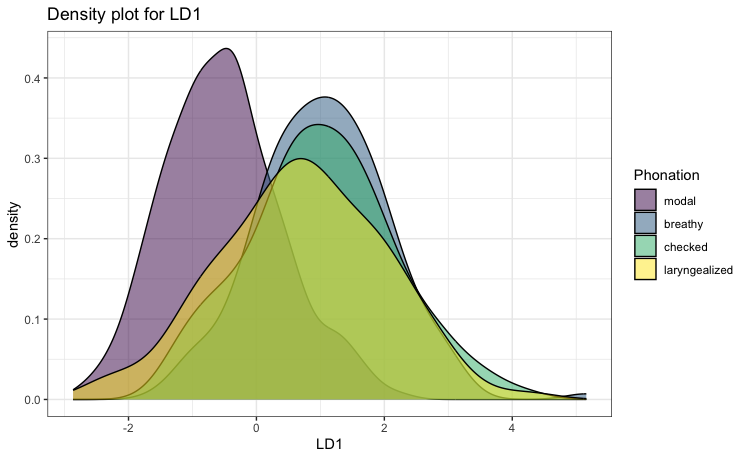
\includegraphics[width=.75\linewidth]{Images/ld1_density.png}
    \caption{Density plot showing LD1 grouped by SLZ's phonation types.}
    \label{fig:LD1}
\end{figure}

LD2 discriminates breathy and checked vowels from the other phonation types and is most strongly associated with HNR \textless 2500 Hz and SoE. HNR \textless 500 Hz is also strongly associated with LD2; see Figure~\ref*{fig:LD2}. 
\begin{figure}[!h]
    \centering
    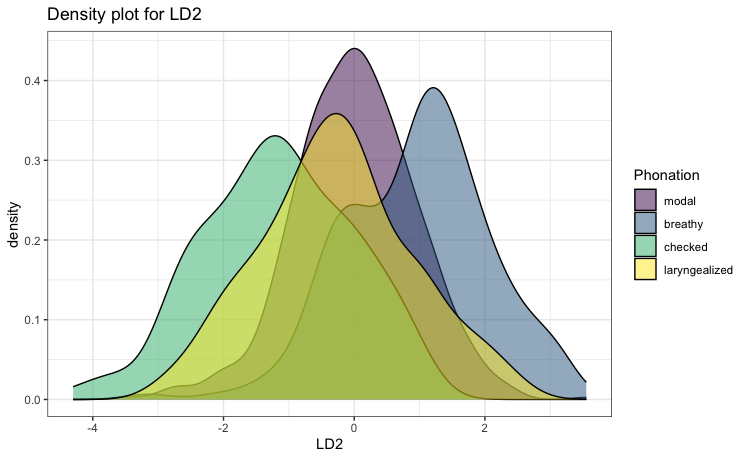
\includegraphics[width=.75\linewidth]{Images/ld2_density.png}
    \caption{Density plot for LD2 grouped by SLZ's phonation types.}
    \label{fig:LD2}
\end{figure}

LD3 discriminates laryngealized vowels from the other phonation types and is also highly associated with the same measures as LD1 except for SoE, which is instead replaced by $\Delta$HNR \textless 2500 Hz (end), which represents the difference in HNR \textless 2500 Hz from the middle to the end of the vowel; see Figure~\ref*{fig:LD3}. 
\begin{figure}[!h]
    \centering
    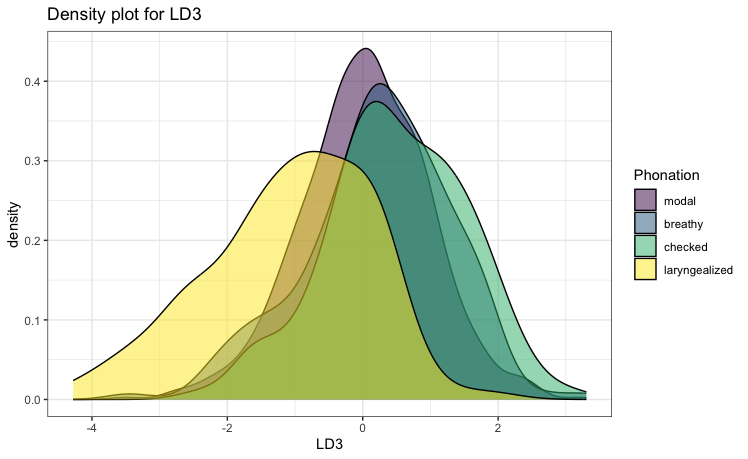
\includegraphics[width=.75\linewidth]{Images/ld3_density.png}
    \caption{Density plot for LD3 grouped by SLZ's phonation types.}
    \label{fig:LD3}
\end{figure}


%------------------------------------
\subsection{Statistical results on the output of the LDA} \label{sec:Stats}
%------------------------------------

The five resulting acoustic measures from the LDA were then analyzed for statistical significance through a mixed-effects linear regression using R's lme4 package \citep{batesFittingLinearMixedEffects2015}. The acoustic measures were treated as the dependent variable in each linear regression model, with phonation as the predictor. The interaction between speaker and phonation was treated as a random variable, as was each of the token words.\footnotetext{DV \thicksim Phonation + (Phonation|Speaker) + (1|Word)} When evaluating the mixed-effects linear regression models, the modal vowel was also treated as the intercept of the model. This means the regression model results for each non-modal phonation type are made to the modal vowel.  

The first linear discriminant function was most strongly affected by HNR\textless 2500 Hz, HNR\textless 3500 Hz, and Strength-of-Excitation. The two HNR measures are associated with measures of periodicity but in different bandwidths. HNR\textless 2500 Hz is concerned with measuring periodicity below 2500 Hz. Because non-modal phonation is associated with aperiodicity, we expect the values for breathy, checked, and laryngealized vowels to be lower than those for modal vowels. As we see in Figure~\ref*{fig:HNR25}, the values for breathy, checked, and laryngealized vowels are all lower than the modal vowels. 
\begin{figure}[!h]
	\centering
	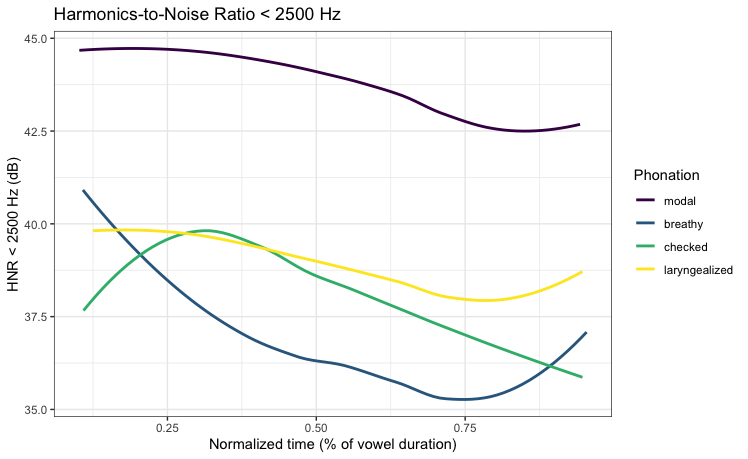
\includegraphics[width=.75\linewidth]{Images/HNR25.png}
	\caption{Line graph showing the change of HNR\textless 2500 Hz across the vowels grouped by SLZ's phonation types.}
	\label{fig:HNR25}
\end{figure}

When we turn to the mixed-effects linear regression model for HNR<2500 Hz, we observe that all three values will change negatively to the modal's values for every step of change in modal vowels. However, only the changes in breathy and checked vowels are significant; see Table~\ref*{tab:HNR25}.
\begin{table}[!h]
    \centering
    \caption{Results of the mixed-effects linear regression analysis for HNR < 2500 Hz.}
    \label{tab:HNR25}
    \begin{tabular}{lrrrrrl}
	\lsptoprule
					&  Estimate  & Std. Error & df & t value & p-value & \\
        \textit{Modal}  &  0.1347	& 0.0558 & 151.5648 &  2.414 & 0.01696 & * \\  
  	Breathy   		&  -0.4914 	& 0.1530 &  9.9072  & -3.213 & 0.00939 & ** \\
	Checked    		&  -0.4669  & 0.1769 &  6.6601  & -2.640 & 0.03499 & * \\
	Laryngealized	&  -0.1654  & 0.1810 & 17.8292  & -0.914 & 0.37293 & \\
    \lspbottomrule
    \end{tabular}
\end{table}

When we turn to the acoustic measure HNR<3500 Hz, which measures periodicity below 3500 Hz, we see that the three non-modal phonation types all show lower values than modal vowels; see Figure~\ref*{fig:HNR35}. Similar to HNR<2500 Hz, these lower HNR values indicate that these phonation types show aperiodicity in their production. 
\begin{figure}[!h]
	\centering
	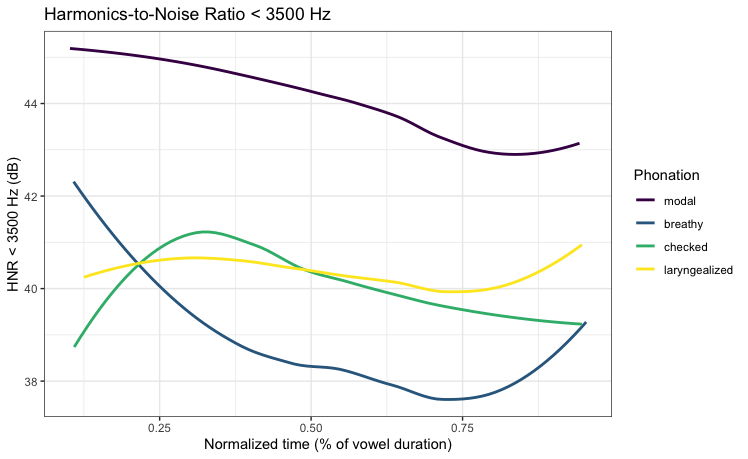
\includegraphics[width=.75\linewidth]{Images/HNR35.png}
	\caption{Line graph showing the change of HNR\textless 3500 Hz across the vowels grouped by SLZ's phonation types.}
	\label{fig:HNR35}
\end{figure}

In contrast to the mixed-effect linear regression model for HNR<2500 Hz, the mixed-effects linear regression for HNR\textless 3500 Hz shows that the differences we observe between the non-modal phonation types and the modal vowels are not statistically significant; see Table~\ref*{tab:HNR35}. 
\begin{table}[!h]
    \centering
    \caption{Results of the mixed-effects linear regression analysis for HNR < 3500 Hz.}
    \label{tab:HNR35}
    \begin{tabular}{lrrrrrl}
	\lsptoprule
					&  Estimate  & Std. Error & df & t value & p-value & \\
        \textit{Modal}  &   0.10018  &  0.05403 & 150.80549 &  1.854 &  0.0657 & . \\  
  	Breathy   		&  -0.33967  &  0.15350 &  9.77806  &-2.213 &  0.0519 & . \\
	Checked    		&  -0.37542  &  0.17313 &  6.62514  &-2.168 &  0.0690 & . \\
	Laryngealized	&  -0.09672  &  0.16999 & 20.16718  &-0.569 &  0.5757 & \\
    \lspbottomrule
    \end{tabular}
\end{table}

The last acoustic measure strongly associated with the first linear discriminant function was Strength-of-Excitation, a measure of the intensity of voicing regardless of the noise in the signal. This SoE measure means that the closer the value is to zero, the less intense the voicing is and indicates a constriction closure to the glottis \citep{mittalStudyEffectsVocal2014,garellekVoicingGlottalConsonants2021}. When we consider the same type of graph showing the SoE values for each of the different phonation types across the vowel, we see that modal vowels have the highest SoE values across the length of the vowel, which is consistent with it lacking a glottal gesture; see Figure~\ref{fig:SOE}. However, what is interesting to see is that checked vowels begin at roughly the same height as modal vowels for SoE. Still, as the length of the vowel increases, the checked vowels progressively have lower and lower SoE values until becoming the lowest at the end of the vowel. Both breathy and laryngealized also exhibit a lower SoE value than modal phonation, which is consistent with having glottal gestures.

\begin{figure}[!h]
	\centering
	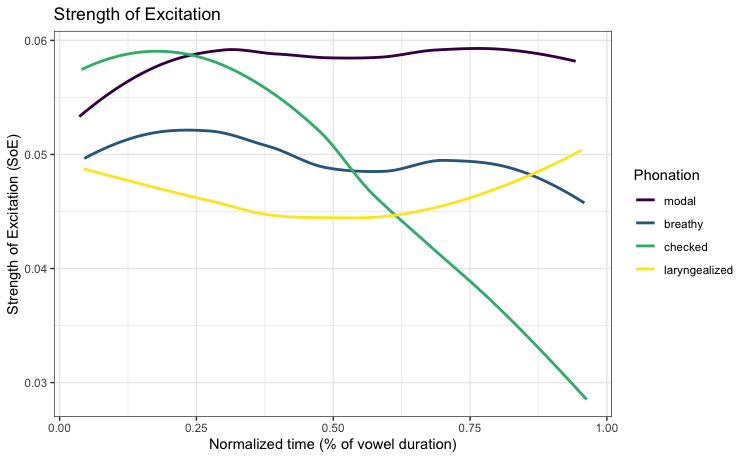
\includegraphics[width=.75\linewidth]{Images/SoE.png}
	\caption{Line graph showing the change of Strength-of-Excitation across the vowels grouped by SLZ's phonation types.}
	\label{fig:SOE}
\end{figure}

When evaluating this measure with a mixed-effects linear regression model, we observe that the changes in SoE across all non-modal phonation types are statistically significant; see Table~\ref{tab:SOE}. 

\begin{table}[!h]
    \centering
    \caption{Results of the mixed-effects linear regression analysis for SoE.}
    \label{tab:SOE}
    \begin{tabular}{lrrrrrl}
	\lsptoprule
					&  Estimate  & Std. Error & df & t value & p-value & \\
        \textit{Modal}  &   0.65006  &  0.04328 &  5.33922 & 15.018 & 1.43e-05 & *** \\  
  	Breathy   		&  -0.11532  &  0.03057 &  7.41179 & -3.772 & 0.006265 & ** \\
	Checked    		&  -0.11516  &  0.02230 &  9.38943 & -5.165 & 0.000517 & *** \\
	Laryngealized	&  -0.08573  &  0.03299 & 11.87923 & -2.599 & 0.023424 & * \\
    \lspbottomrule
    \end{tabular}
\end{table}

The second linear discriminant function was similarly associated with HNR\textless 2500 Hz and SoE like they were for the first linear discriminant function. Instead of HNR\textless 3500 Hz, a different HNR measure strongly affected this second linear discriminant function. HNR\textless 500 Hz measure periodicity below 500 Hz. Figure~\ref{fig:HNR05} shows that, like the other HNR measures, all three non-modal phonation types show a lower HNR value consistent with them being aperiodic. However, when the mixed-effects linear regression model was run on the acoustic measure, the only checked phonation reached significance; see Table~\ref{tab:HNR05}. 

\begin{figure}[!h]
	\centering
	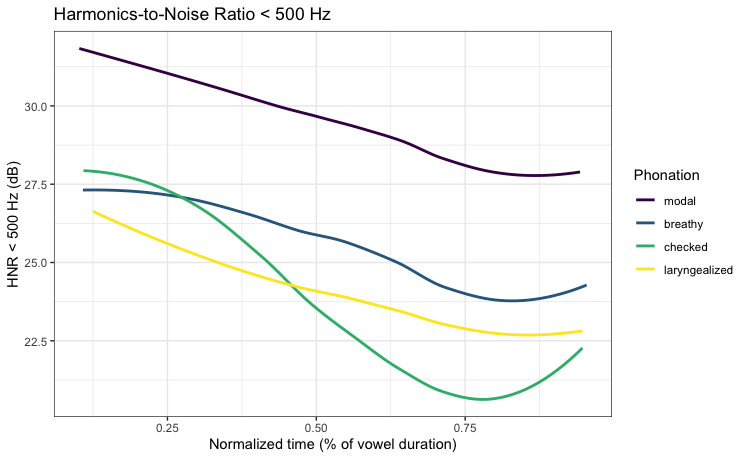
\includegraphics[width=.75\linewidth]{Images/HNR05.png}
	\caption{Line graph showing the change of HNR < 500 Hz across the vowels grouped by SLZ's phonation types.}
	\label{fig:HNR05}
\end{figure}

\begin{table}[!h]
    \centering
    \caption{Results of the mixed-effects linear regression analysis for HNR < 500 Hz.}
    \label{tab:HNR05}
    \begin{tabular}{lrrrrrl}
	\lsptoprule
					&  Estimate  & Std. Error & df & t value & p-value & \\
        \textit{Modal}  &  0.14980  & 0.07553 & 9.64369 &  1.983 & 0.07652 & . \\  
  	Breathy   		&  -0.05906 & 0.20426 & 6.38671 & -0.289 & 0.78162 &  \\
	Checked    		&  -0.70904 & 0.16811 & 6.77873 & -4.218 & 0.00424 & ** \\
	Laryngealized	&  -0.29020 & 0.23947 & 7.58130 & -1.212 & 0.26197 & \\
    \lspbottomrule
    \end{tabular}
\end{table}

The third linear discriminant function only introduced one new acoustic measure. $ \Delta $HNR<2500 Hz (end) measures the difference between the middle and end of the vowel for HNR\textless 2500 Hz. As seen in Figure~\ref{fig:HNR25}, the HNR measure changes most drastically from the middle of the vowel to the end of the vowel for checked phonation. The other phonation types also change but do not change as quickly. The difference can be seen in Figure~\ref{fig:HNR25} when we compare the values in the middle portion of the graph to those at the end for each phonation type. This magnitude of change is reflected in the linear regression for $ \Delta $ HNR<2500 Hz (end), with checked phonation being the only one that showed actual statistical significance; see Table~\ref{tab:delta}. 

\begin{table}[!h]
    \centering
    \caption{Results of the mixed-effects linear regression analysis for $ \Delta $HNR<2500 Hz (end).}
    \label{tab:delta}
    \begin{tabular}{lrrrrrl}
	\lsptoprule
					&  Estimate  & Std. Error & df & t value & p-value & \\
        \textit{Modal}  &   -0.02397 &   0.06574  & 32.69794 & -0.365 & 0.71774 & \\  
  	Breathy   		&    0.12279 &   0.14446  & 11.41768 &  0.850 & 0.41280 & \\
	Checked    		&    0.32531 &   0.10589  & 41.57481 &  3.072 & 0.00374 & ** \\
	Laryngealized	&   -0.12616 &   0.27805  &  8.21579 & -0.454 & 0.66176 & \\
    \lspbottomrule
    \end{tabular}
\end{table}

%------------------------------------
\section{Discussion} \label{sec:Discussion}
%------------------------------------

%------------------------------------
\subsection{Linear discriminant analysis discussion} \label{sec:DiscussionLDA}
%------------------------------------
The results of the linear discriminant analysis showed that the acoustic measures used in the PMoP are sufficient to account for the different phonation types in SLZ. The linear discriminant analysis performed well above chance at 70.45\%. The linear discriminant analysis further showed that each of the four could be discriminated by the three discriminant functions it produced. However, as mentioned above in Section~\ref{sec:LDAResults}, the linear discriminant analysis performed better at classifying some phonation types over others. The model could classify modal vowels best at almost 90\% accuracy; breathy vowels at 45\%; checked at 37\%; and laryngealized at 22\%. The confusion matrix in Table~\ref{tab:Confusion} shows that all nonmodal phonation types were predominantly confused with modal vowels. This is not too unsurprising because of the highly variable nature in which these nonmodal phonation types are produced. 

The linear discriminant analysis additionally showed that the acoustic measures that contributed the most to the three linear discriminant functions were harmonic-to-noise ratios along three different bandwidths and strength-of-excitation. Even though these acoustic measures had the greatest association, it does not mean that these are the only measures necessary to understand the phonation contrasts. Each linear discriminant function comprises a linear combination of all the acoustic measures and their associated coefficient. In more phonological terms, we can imagine these linear discriminant functions similar to the formula phonologists use to derive each candidate's harmonic score within Harmonic Grammar \citep{smolenskyHarmonicMindNeural2006}. In Harmonic Grammar, each constraint contributes weight to the formula, with some constraints contributing a greater weight and others a lower weight; a linear discriminant function assigns a numerical coefficient to each acoustic measure. Just because one acoustic measure has a lower coefficient does not mean an acoustic measure is not important to how speakers produce or perceive the phonation contrasts in Zapotec. A combination of several low-weighted acoustic measures may produce enough ``weight" to overcome the ``weight" of these heavier harmonic-to-noise ratios, similar to gang effects in Harmonic Grammar. 

Instead of using the absolute value of the coefficients in the linear discriminant functions to determine which acoustic measures are to consider, another method is to take the mean predictive value of the three linear discriminant functions and determine the correlation values for each acoustic measure within each linear discriminant function. This is the method used by \citet{garellekAcousticDiscriminabilityComplex2020} for determining which acoustic measures to use in his analysis for !Xóõ. 

Both methods have their merits, but using the coefficients of the acoustic measures instead of their correlations is in line with more general practices used in the statistical literature. Different acoustic measures have the strongest correlation when using this other method with this study's linear discriminant analysis. The three highest acoustic measures according to absolute correlation score for each linear discriminant function are reported in Table~\ref{tab:LDA2}. Evaluating these measures will be left for further analysis. 

\begin{table}[!h]
    \centering
    \caption{Acoustic measures with the highest absolute correlations for the three linear discriminant functions.}
    \label{tab:LDA2}
    \begin{tabular}{lll}
	\lsptoprule
	LD1  & LD2 & LD3  \\
	\hline
    \begin{tabular}[c]{@{}l@{}}SoE \\ $f0$ \\ HNR < 1500 Hz\end{tabular} & \begin{tabular}[c]{@{}l@{}}$f0$\\ $\Delta$SoE (end)\\ B1\end{tabular} & \begin{tabular}[c]{@{}l@{}}$\Delta$SoE (end)\\ $\Delta$F3 (end)\\ $\Delta$HNR \textless 1500 Hz (beg)\end{tabular} \\
    \lspbottomrule
    \end{tabular}
\end{table}

%------------------------------------
\subsection{Harmonic-to-noise ratio discussion} \label{sec:DiscussionHNR}
%------------------------------------

As previously mentioned, the acoustic measures that contributed the most ``weight" to the three linear discriminant functions were predominantly harmonic-to-noise ratios across three different bandwidths. Out of the three harmonic-to-noise ratios that the linear discriminant functions called out, all were highly significant for at least one non-modal phonation, except for HNR\textless 3500 Hz. This acoustic measure never reached significance; however, the \textit{p}-value for the breathy and checked non-modal phonations hovered very close to the alpha value of 0.05. HNR\textless 3500 Hz was not as informative because it subsumes the narrower bandwidths of \textless 500 Hz and \textless 2500 Hz with its wider bandwidth of \textless 3500 Hz. It is also important to remember that under the Psychoacoustic Model of Phonation (PMoP; \cite{kreimanUnifiedTheoryVoice2014}), a single acoustic measure is not more important than another, but the acoustic measures associated with the harmonic spectral slopes, the inharmonic source noise, the time-varying source characteristics, and the vocal tract transfer functions combined together tell a complete story of how phonation is produced in a language. 

When relying on the coefficient values, the ``delta" score contributed little to the linear discriminant functions. This result is surprising, considering how the different phonation types behave dynamically, especially when distinguishing between laryngealized and checked vowels. One reason for this could be the same sample size reported in this paper of six speakers. It is very likely that the data from the remaining 12 speakers could improve the model and show the importance of these ``delta" scores. However, when we consider the correlation of the mean predictive value of the linear discriminant function and the acoustic measures instead of the ``weights", as shown in Table~\ref{tab:LDA2} above, these ``delta" scores make up the three highest correlations for the third linear discriminant function and the second highest correlation in the second linear discriminant function. This suggests that depending on evaluating by correlation of the linear discriminant functions and their component variables or evaluating the raw ``weight" of the acoustic measures could produce different outcomes. Accounting for why this is beyond the scope of this paper but will be left for further research. 

%------------------------------------
\subsection{Laryngealized vowel discussion} \label{sec:DiscussionLaryngealized}
%------------------------------------

When we focus on how well the linear discriminant analysis performed at classifying the different acoustic measures, we notice that the model did very poorly for laryngealized vowels, which the linear discriminant analysis performed the worst on at 22\% chance, which is below chance. As mentioned above in Section~\ref{sec:SLZ}, laryngealized vowels show the greatest variability in their production inter- and intra-speaker. For some productions of this vowel, speakers would produce a vowel with model phonation throughout its entirety. The only indication that the vowel was non-model was a small period of two to three glottal pulses that had a lower amplitude than the rest of the vowel, very similar to what \citet{gerfenProductionPerceptionLaryngealized2005} found for laryngealized vowels in Mixtec. At other times, the production was with a tense voice rather than a canonical creaky voice. 

Another aspect of laryngealized voice that the linear discriminant analysis revealed is that 

%------------------------------------
\subsection{Laryngeal Complexity Hypothesis} \label{sec:LCH}
%------------------------------------
Another question has to do with the predictions from the Laryngeal Complexity Hypothesis. The \textsc{Laryngeal Complexity Hypothesis} (LCH) has its origins in work by \citet{silvermanLaryngealComplexityOtomanguean1997,blankenshipTimeCourseBreathiness1997,blankenshipTimingNonmodalPhonation2002}. The basic premise of the LCH is that in languages that have both tone and phonation, there needs to be an ordering between the two laryngeal gestures for tone and phonation for optimal perceptibility. This premise comes from the understanding that the same mechanism responsible for tone is also responsible for the production of phonation: the vocal folds and glottis. The rate at which vocal folds vibrate is responsible for changing the fundamental frequency, perceived as pitch, which is grammaticalized as tone in lexical tone languages. The faster the vocal folds vibrate, the higher the pitch. And the slower the vocal folds vibrate, the lower the pitch. 

The vocal folds are also the primary articulator for phonation. \citet{ladefogedPreliminariesLinguisticPhonetics1971,gordonPhonationTypesCrosslinguistic2001} treated phonation as a by-product of how open or closed the glottis is during vocal fold vibration. This is schematized by Figure~\ref{fig:Phonation}. The more open the glottis is, the breathier the sound to the point where the sound becomes the sound [h]. The more closed the glottis is, the creakier the sound is to the point where the sound becomes [ʔ]. 

\begin{figure}[!ht]
	\centering
	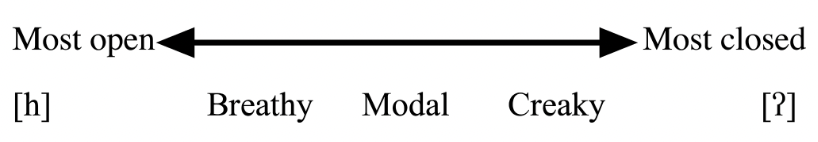
\includegraphics[width=.6\textwidth]{Phonation.png}
	\caption{One-dimensional model for phonation. Based on \citet{ladefogedPreliminariesLinguisticPhonetics1971,gordonPhonationTypesCrosslinguistic2001}}.
	\label{fig:Phonation}
\end{figure}

The LCH assumes phonation and tone are produced at the vocal folds and glottis. Because these same organs are responsible for these two phenomena, a mismatch exists in trying to have both simultaneously. It is assumed by the LCH that because of this issue, there needs to be strict ordering in the glottal gestures. This means the tonal gesture must be produced before or after the phonation gesture. The reason for this is that if the gestures overlap, there will be a perturbation of the tone, and the listeners will not be able to differentiate the tone reliably. The LCH assumes that there is a close link between production and perception. This assumption places the responsibility on making sure the acoustic cues are the most perceptually salient on the speaker. The speaker is responsible for producing both tone and phonation so that the listener can differentiate the different cues for both tone and phonation. These assumptions can best be represented by Figure~\ref{fig:GlottalGestures}. 

In Figure~\ref{fig:GlottalGestures}, which is taken from \citet{dicanioCoarticulationToneGlottal2012}, the cue for tone is represented by the Pitch Target and the Glottal Gesture represents the gestures needed to produce phonation. When the Pitch Target is not co-articulated with the Glottal Gestures, there is the greatest perceptual recoverability for the listener. The LCH argues for this as the tones are the most recoverable on modal vowels. This modal portion is then ordered or phased relative to the non-modal portion. This ordering is the speaker's responsibility to accommodate the listeners' perceptibility. If, however, the Pitch Target and the Glottal Gesture were overlapping, as represented by the lower half in Figure~\ref{fig:GlottalGestures}, then the cues for pitch and phonation would be overlapping and making it perceptually more difficult for 
\begin{figure}[!ht]
	\centering
	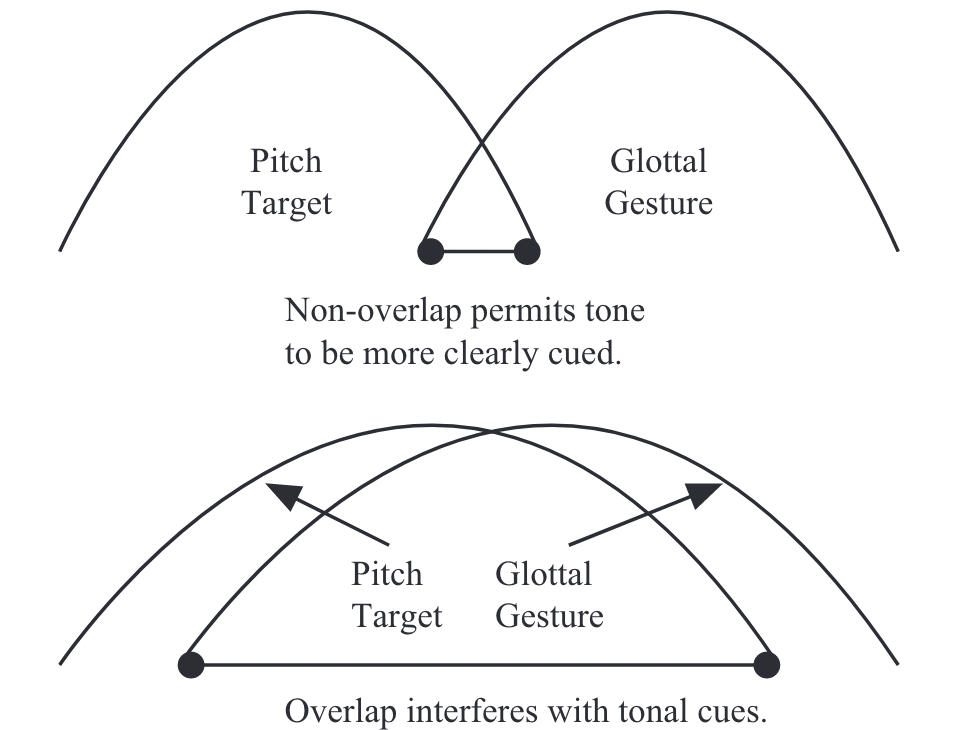
\includegraphics[width=.5\textwidth]{Gestures.png}
	\caption{Representation taken from \citet{dicanioCoarticulationToneGlottal2012}.}
	\label{fig:GlottalGestures}
\end{figure}

Some work has been done investigating this in other languages, most notably \posscitet{dicanioCoarticulationToneGlottal2012} investigation into glottals in Itunyoso Trique, which is also an Oto-Manguean language. \citeauthor{dicanioCoarticulationToneGlottal2012} in his study found that when the magnitude of coarticulation for glottal consonants occurs on the vowels, there is a strong correlation between the magnitude of overlap and the amount of perturbation in the f0 signal. If the degree of overlap was minor, then the acoustic signal had little to no perturbation. These results were found by consulting the spectral tilt of the vowels with the f0 measures and performing a generalized linear mixed effects model with the speaker treated as a random effect. 

Another study on Jalapa Mazatec \citep{garellekAcousticConsequencesPhonation2011} also investigated the interaction of tone and phonation. Jalapa Mazatec is a language with both contrastive tone and phonation, and \citet{garellekAcousticConsequencesPhonation2011} validated the claims made by the LCH, in that tone and phonation seemed to be ordered with each other when it comes to at least one of the phonation types. 

This paper describes the tonal and phonation inventories in Santiago Laxopa Zapotec, an ideal language for testing the viability of the LCH because of its use of both contrastive tone and contrastive phonation.   

Another question this study raises is the status of laryngealized vowels and their realizations. We observed from just two speakers that these vowels are highly variable. Assuming that \posscitet{avelinoAcousticElectroglottographicAnalyses2010} observations on this vowel in the closely related Yalálag Zapotec hold in SLZ, there is considerably more variation that exists within and between speakers. Suppose all of these varying realizations of a phonological category are evident. What does this mean for this category's status and the cues necessary for speakers to produce and realize this category? 

%------------------------------------
\section{Further directions and Conclusions} \label{sec:Conclusion}
%------------------------------------

In conclusion, this paper has briefly introduced the tonal and phonation systems of Santiago Laxopa Zapotec, an understudied variety of Sierra Norte Zapotec. This system is essential for exploring the acoustic cues used in different languages to differentiate each phonation type.

Contrary to acoustic work on other Zapotec varieties by \citet{espositoVariationContrastivePhonation2010}, which showed that female speakers' phonation contrasts were best characterized by H1-H2 and male speakers' contrasts by H1-A3, SLZ suggests that both male and female speakers' breathy voice is best described by H1-A3 and checked and laryngealized voice are characterized by a difference in the timing of spectral-tilt measurements and CPP values depending on the speaker. 

Because of these phonation type differences in behavior, one could, in theory, speak to how SLZ compensates for using the larynx for both tone and phonation. This paper has not explicitly spoken on this issue, and the Laryngeal Complexity Hypothesis presented by \citet{silvermanLaryngealComplexityOtomanguean1997} and \citet{blankenshipTimeCourseBreathiness1997, blankenshipTimingNonmodalPhonation2002}. The LCH states that when a language has tone and phonation, these different aspects are ordered or phased concerning one another. This phasing allows for the most significant perceptibility in the acoustic signal. This allows the listener to interpret the acoustic signals for tone and phonation adequately. 

Overall, there seems to be some information from the spectral-tilt and CPP analysis that speaks to the question of the LCH. If the reader recalls, CPP was the most important cue for differentiating checked and laryngealized vowels from modal and breathy vowels for FSR. The key is the lower CPP value, which corresponds to greater aperiodicity. It is worth repeating that we did see a difference in the timing of the aperiodicity between checked and laryngealized vowels. In laryngealized vowels, this dip in CPP occurs in the middle third of the vowel, and for checked vowels, this dip occurs in the final third. However, the fact that for breathy vowels, the most noticeable cue is the higher H1-A3 which happens throughout the entire vowel, might suggest that breathiness does not behave in the same way as the other phonation types. The behavior from checked and laryngealized vowels seems to support the LCH. Unfortunately, no firm conclusions can be made about the LCH, and further investigation is required to determine the validity of the LCH in SLZ. 

This ability of speakers to interpret the acoustic signals in conjunction with the acoustic signals for tone is of great interest. It would benefit from a perception experiment to determine what the speakers are using to differentiate the different phonation types. This is especially true for laryngealized vowels, which have such varied pronunciations. 

This study will benefit from further analysis and data collection. Now that the world is safer regarding COVID-19, collecting data from more speakers is essential to corroborate the data and analysis from FSR and RD. 

%------------------------------------
%BIBLIOGRAPHY
%------------------------------------

%\singlespacing
% \nocite{*}
\printbibliography[heading=bibintoc]

\end{document}